\documentclass{article}
\usepackage[utf8]{inputenc}
\usepackage{graphicx}
\usepackage{caption}
\usepackage{subcaption}
\usepackage{amsmath}


\title{Image and Video Processing Lab 4}
\author{Philine Witzig}
\date{November 2020}

\begin{document}

\maketitle
In this report, we investigate the perceived visual quality of different point clouds created through two different point cloud encoders. They are referred to as codec 1 (gwi pcl) and codec 2 (pcc geo color) in this report. Moreover, we look at possible objective metrics and try to identify one which can best describe the subjective results. \\

General notes on the matlab script: when running the matlab script, you will be asked to enter the number of the task you want to test. Enter the numbers $1$ to $3$ in order to test the respective task. 

%---------------------------
% Task 1
%---------------------------

\section{Subjective Quality Assessment}
Performing outlier detection using the algorithm described in ITU-T Recommendation P.913, no outliers could be detected in the dataset. Thus, all computations were executed on the original dataset having $22$ participants. \\

Figure \ref{fig:dmos_br} shows the computed DMOS vs. the bitrate for the two different codecs per content. Furthermore, the confidence intervals were computed with $\alpha=0.05$, leading to a confidence interval of 95\%. Note that the scaling of the x-axis might vary due to different bitrates used for the different models. \\

We can observe similar trends between the different contents in Figure \ref{fig:dmos_br}. Since the DMOS is a measure representing the differential overall quality (visual in our case), one can say that codec 2 (pcc geo color) almost always leads to a better visual quality compared to codec 1 (gwi pcl) for small bitrates. Only if we choose our bitrate to be high for codec 1, the models obtain a visual quality which is comparable to the ones when codec 2 was used (according to the DMOS value). \\

Furthermore, it is worth mentioning that depending on the content, the difference in the rated visual quality between codec 1 and codec 2 varies. For example, for the content \textsf{longdress}, the DMOS curves seem to vary more from each other than for content \textsf{phil}. Thus, the perceived quality not only depends on the codec and the bitrate used but also on the content itself. In terms of the confidence intervals, we can observe that the content \textsf{rethorician} has comparably small confidence intervals. Wider confidence intervals mean that the DMOS is less precise. Thus the agreement on a quality value between subjects also seems to vary with the content. \\

Last but not least, one can observe from Figure \ref{fig:dmos_br} that a high bit rate is not necessarily the key to success. For the \textsf{rhetorician} content, the DMOS drops again for codec 2 when a bitrate of about $4$ is used. \\

Therefore, one can say that the perceived visual quality of a model depends on three factors: the codec, the bitrate and the content itself.

\begin{figure}
\begin{subfigure}[b]{0.49 \textwidth}
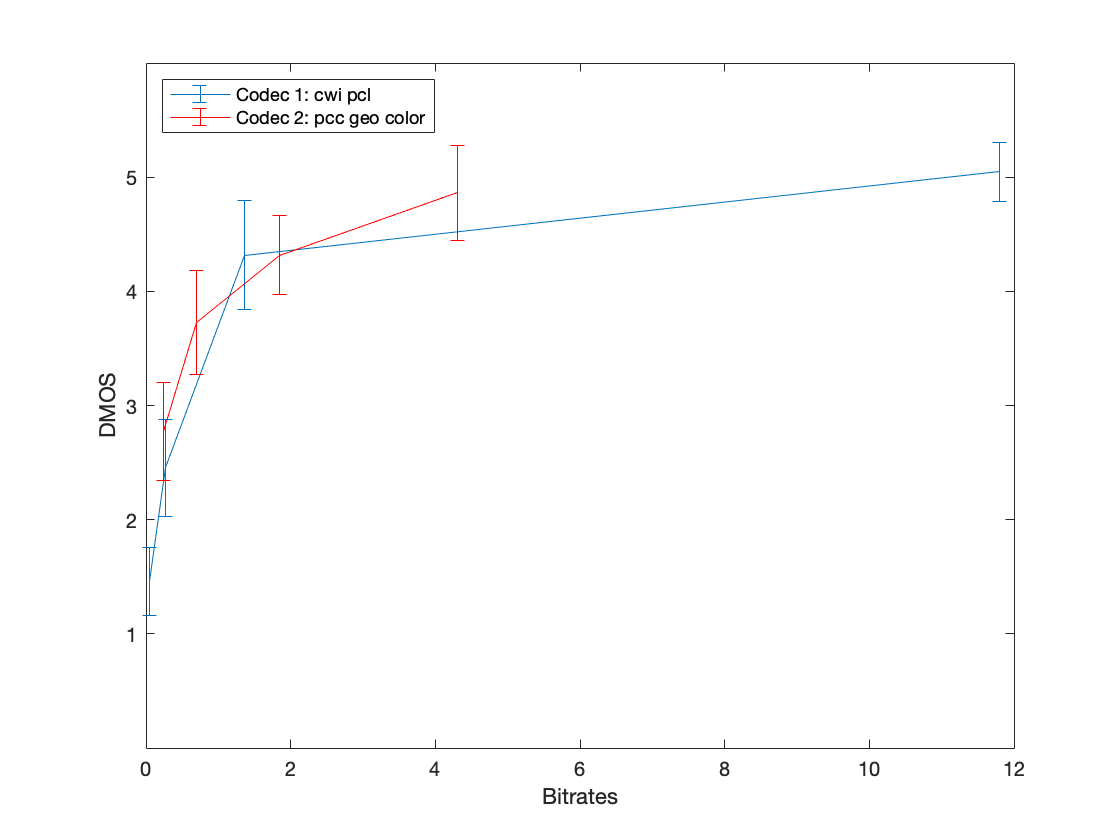
\includegraphics[width=\textwidth]{Figures/task1/dmos_guanyin.png}
\subcaption{\textsf{gunayin}}
\end{subfigure}
\begin{subfigure}[b]{0.49 \textwidth}
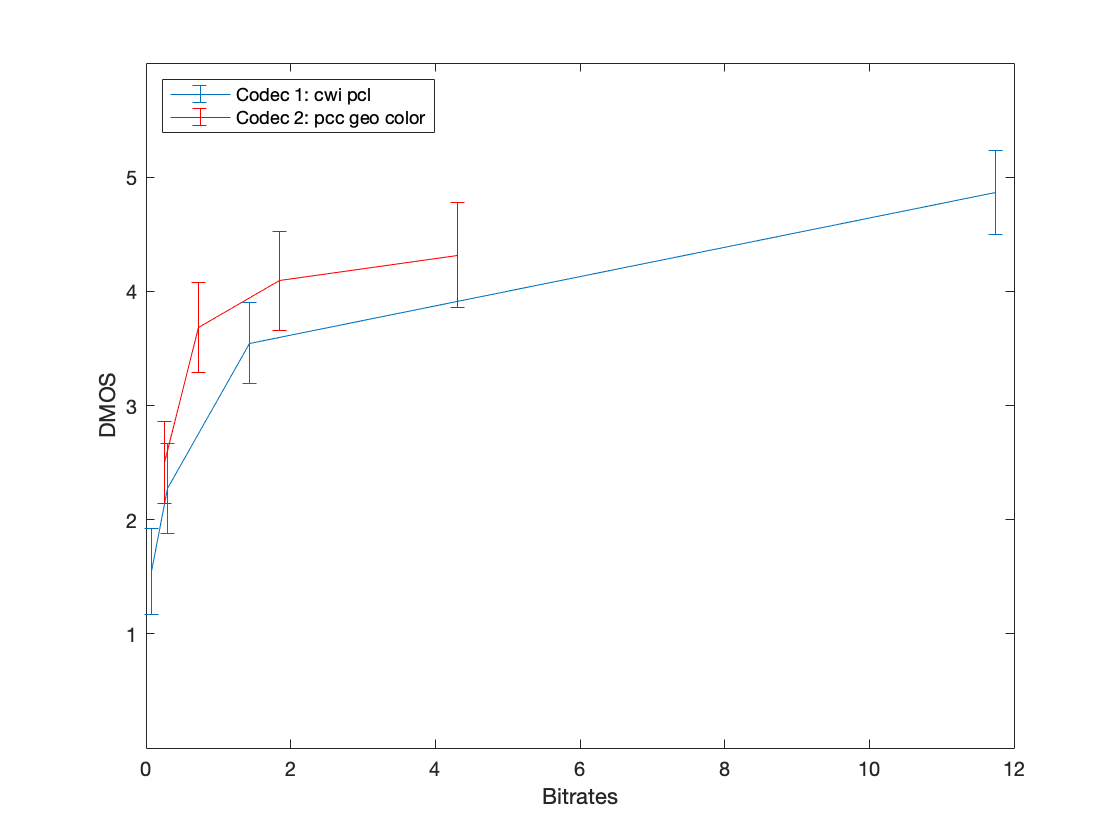
\includegraphics[width=\textwidth]{Figures/task1/dmos_long_dress.png}
\subcaption{\textsf{longdress}}
\end{subfigure}
\begin{subfigure}[b]{0.49 \textwidth}
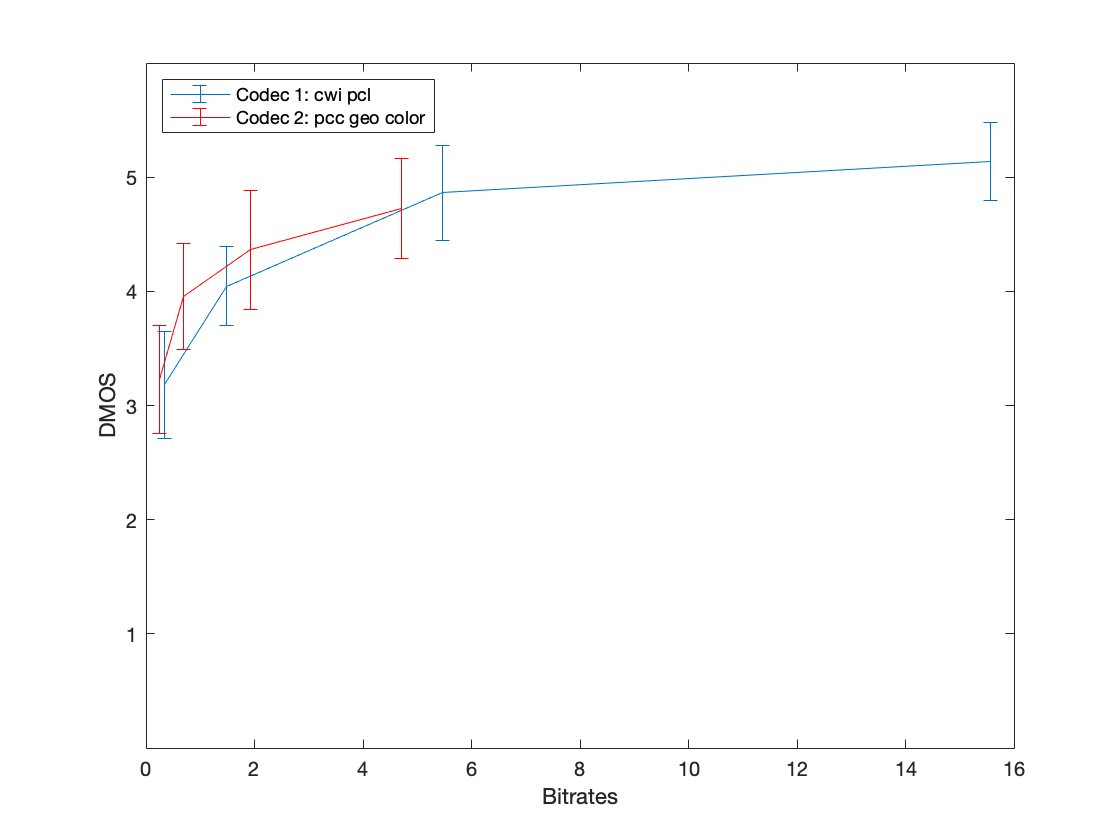
\includegraphics[width=\textwidth]{Figures/task1/dmos_phil.png}
\subcaption{\textsf{phil}}
\end{subfigure}
\begin{subfigure}[b]{0.49 \textwidth}
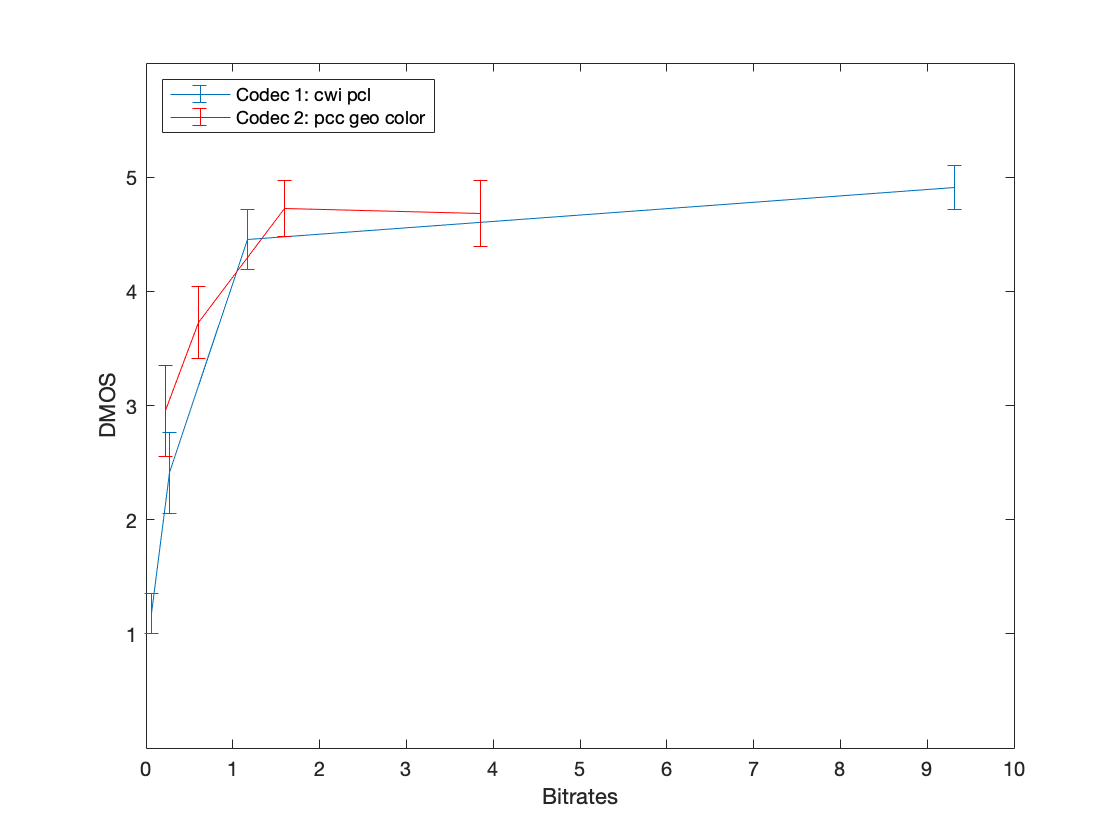
\includegraphics[width=\textwidth]{Figures/task1/dmos_rhetorician.png}
\subcaption{\textsf{rhetorician}}
\end{subfigure}
\caption{DMOS with CI against bitrate for codec 1 (cwi pci) in blue and codec 2 (pcc geo color) in red on the four contents.}
\label{fig:dmos_br}
\end{figure}


\section{Objective Quality Assessment}
In this task, different objective quality metrics are evaluated on the different contents per codec. In particular, we looked at point to point distance using MSE and Hausdorff, plane to plane using angular similarity and color metrics on the RGB space (using equations 14 and 15 from the assignment) and on the YUV space. Figures \ref{fig:obj_guanyin} to \ref{fig:obj_rhetorician} show plots of the objective metric values against the bitrate for each codec per model. Note that the Hausdorff distance is a similarity measure. Thus, the higher its value the lower the introduced error. \\

What we can observe from Figure \ref{fig:obj_guanyin} to Figure \ref{fig:obj_rhetorician} is, that for point to point and plane to plane metrics, we have different trends depending on the content. For content \textsf{guanyin}, both, point to point and plane to plane metrics indicate a lower introduced error compared to when codec 2 (pcc geo color, red curve) was used. This also holds for content \textsf{longdress}. Here, the difference is even stronger than for \textsf{guanyin}. In contrast, for content \textsf{phil}, the point 2 point metric with MSE indicates that with increasing bitrate, the error introduced through codec 1 becomes smaller than for codec 2 while it was the opposite for small bitrates. Such a changing trend is not observable when the point 2 point metric with Hausdorff distance was used. Here, codec 2 seems to introduce a smaller error for all bitrates. Looking at the angular similarity, we observe a conflicting trend for small bitrates. However, for large bitrates codec 1 seems to introduce a smaller error on \textsf{phil}. Last but not least, for \textsf{rhetorician} codec 2 seems to outperform codec 1 in terms of point to point metrics. However, with increasing bitrate codec 1 produces normal vectors which are closer to the reference model compared to codec 2, thus leading to larger angular similarity. \\

 If we compare both codecs using  color metrics, the trends are more consistent between the contents.
 We can observe that a large bitrate leads to a large color error/distortion. For smaller bitrates, codec 2 generally introduces a larger color error than codec 1. Comparing the metrics using different color spaces, it can be seen that the encoders introduce a higher error in the YUV space. Thus, one need to be particularly careful when using both encoders for point clouds which will be displayed on devices making use of the YUV space.\\
 
 To summarize the above findings, one can say that in general, codec 1 produces slightly better color quality than codec 2 for small bitrates. For large bitrates, the opposite holds. In terms of geometric distortion, there does not seem to be one unique trend across the contents for the different codecs. In particular, the objective scores seem to depend on the content itself.  
% Guanyin
\begin{figure}
    \centering
    \begin{subfigure}[b]{0.65\textwidth}
    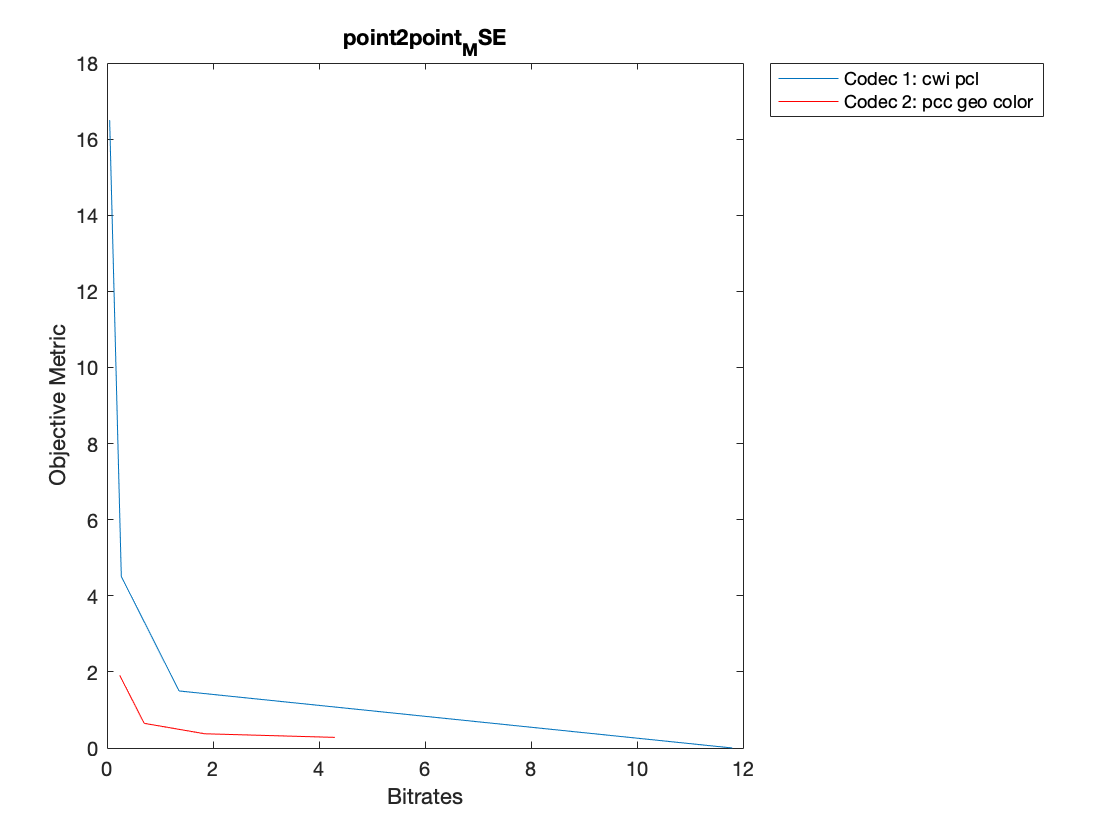
\includegraphics[width=\textwidth]{Figures/task2/guanyin_p2p_mse.png}
    \subcaption{Point to point metric using MSE.}
    \end{subfigure}

    \begin{subfigure}[b]{0.65\textwidth}
    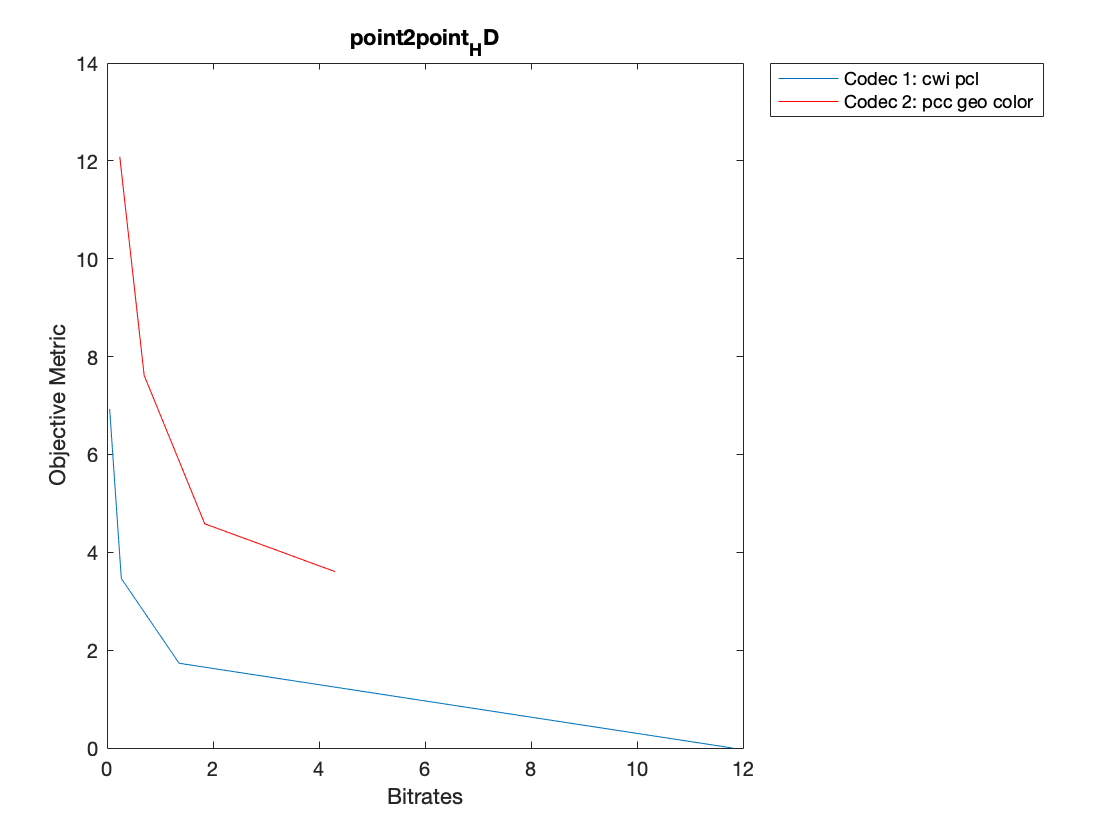
\includegraphics[width=\textwidth]{Figures/task2/guanyin_p2p_hd.png}
    \subcaption{Point to point metric using Hausdorff distance.}
    \end{subfigure}

    \begin{subfigure}[b]{0.65\textwidth}
    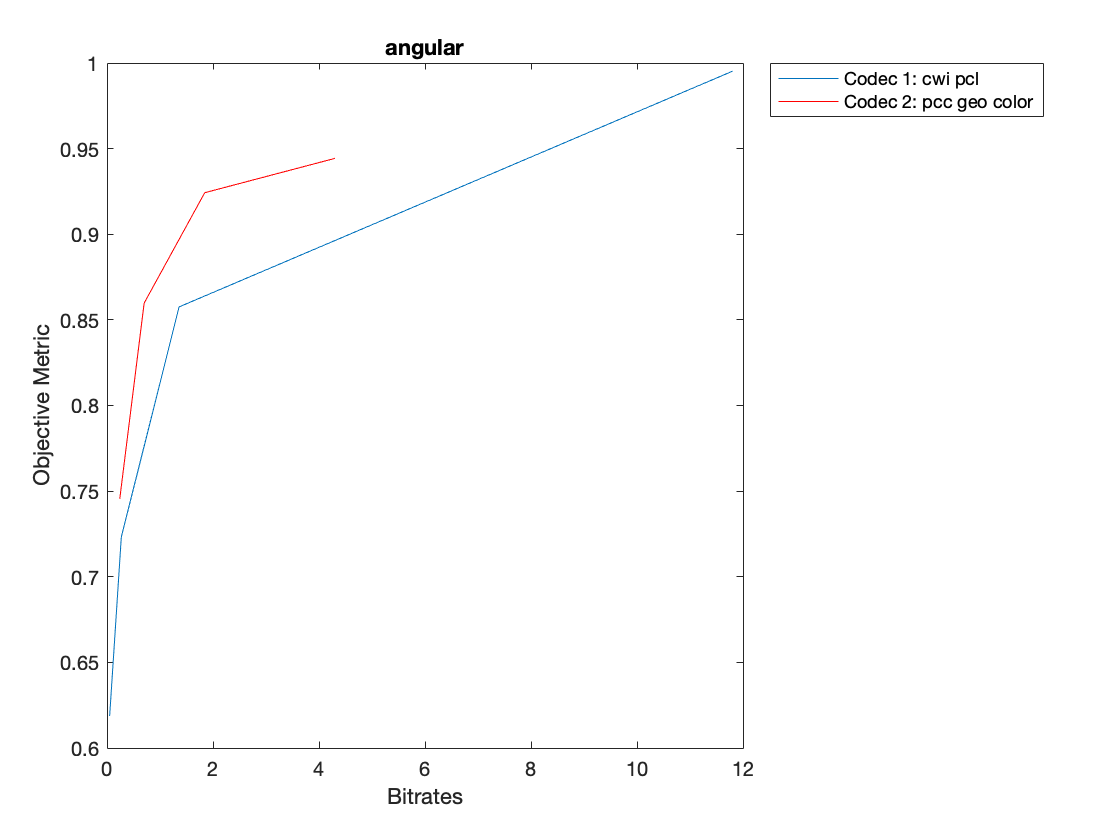
\includegraphics[width=\textwidth]{Figures/task2/guanyin_angular.png}
    \subcaption{Plane to plane metric, computing angular similarity.}
    \end{subfigure}
  
\end{figure}
\begin{figure}
     \ContinuedFloat
    \begin{subfigure}[b]{0.65\textwidth}
    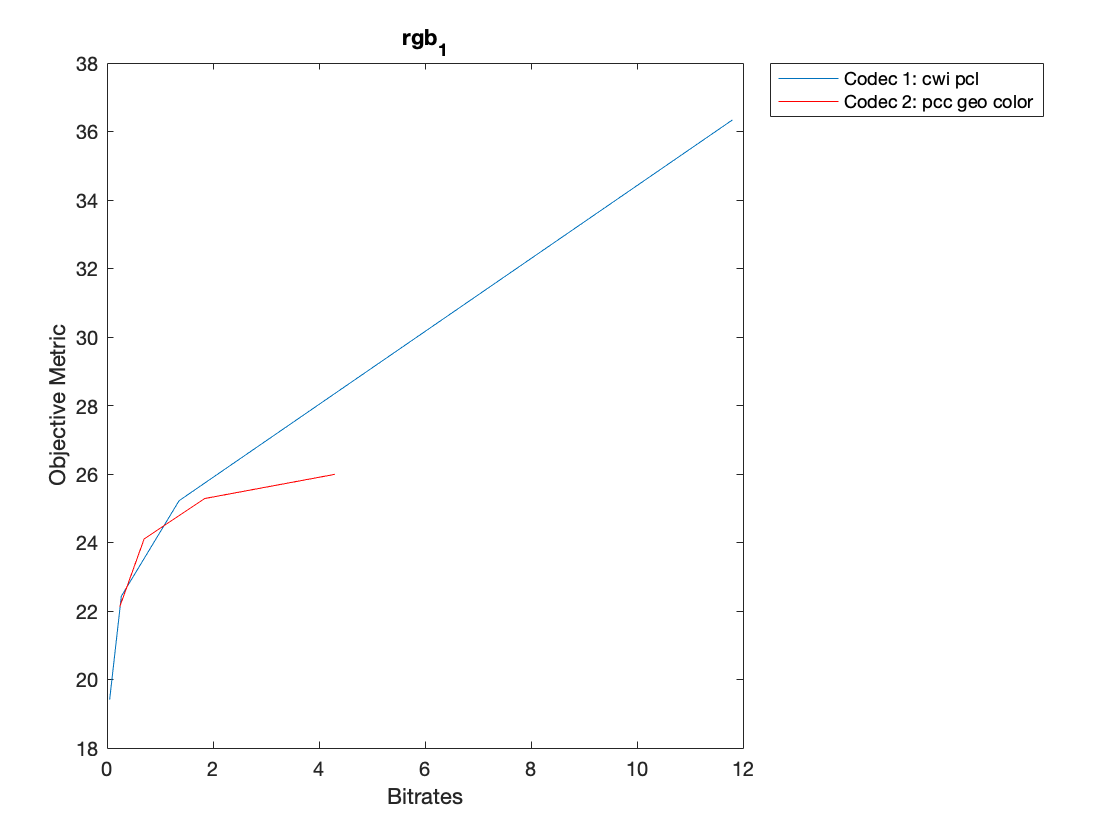
\includegraphics[width=\textwidth]{Figures/task2/guanyin_rgb1.png}
    \subcaption{Symmetric color-PSNR, RGB space using eq. 14.}
    \end{subfigure} 
    \begin{subfigure}[b]{0.65\textwidth}
    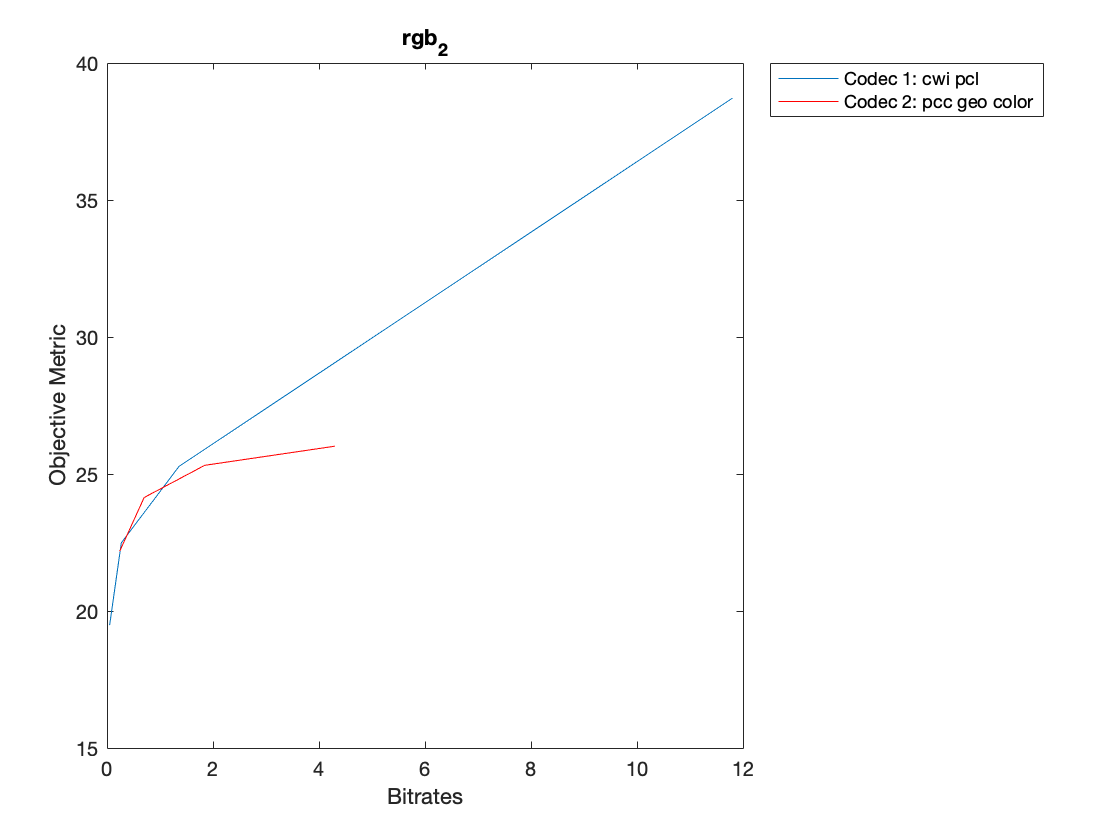
\includegraphics[width=\textwidth]{Figures/task2/guanyin_rgb2.png}
    \subcaption{Symmetric color-PSNR, RGB space using eq. 15.}
    \end{subfigure}
    
    \begin{subfigure}[b]{0.65\textwidth}
    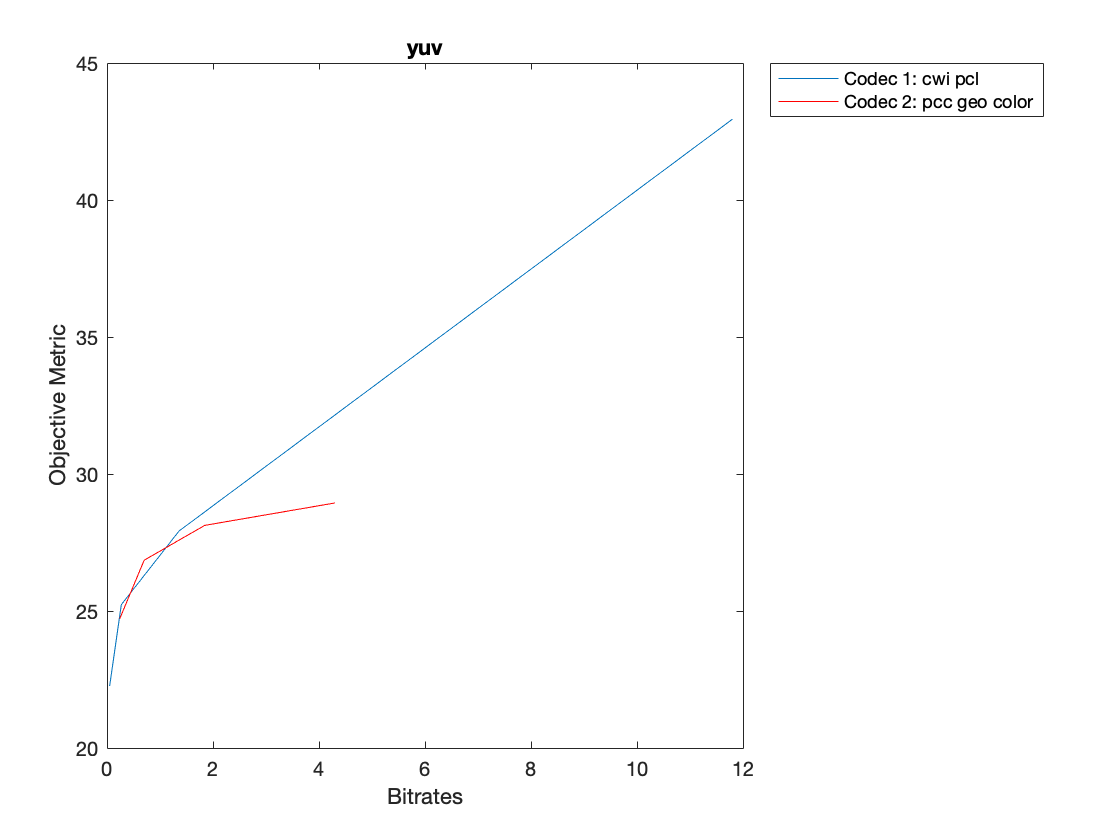
\includegraphics[width=\textwidth]{Figures/task2/guanyin_yuv.png}
    \subcaption{Symmetric color-PSNR, YUV space.}
    \end{subfigure}
    \caption{Objective quality assessment on \textsf{guanyin} point cloud.}
    \label{fig:obj_guanyin}
\end{figure}

% Longdress
\begin{figure}
    \centering
    \begin{subfigure}[b]{0.65\textwidth}
    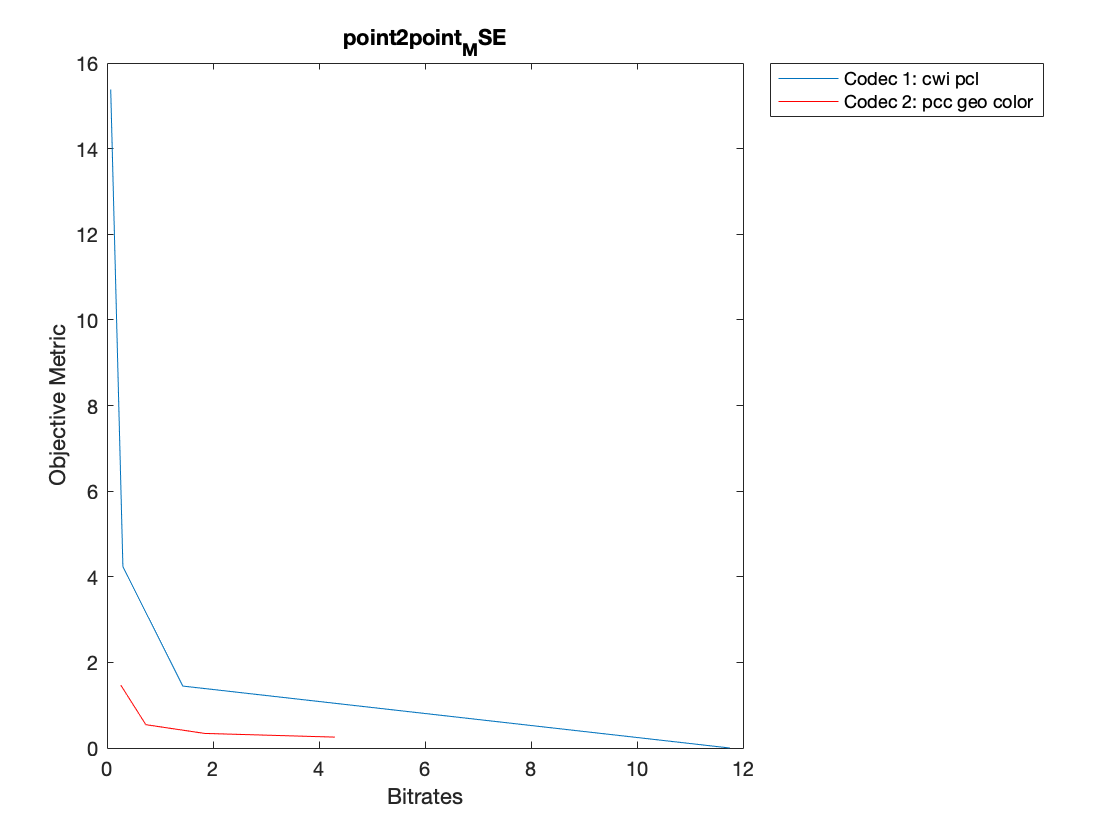
\includegraphics[width=\textwidth]{Figures/task2/longdress_p2p_mse.png}
    \subcaption{Point to point metric using MSE.}
    \end{subfigure}

    \begin{subfigure}[b]{0.65\textwidth}
    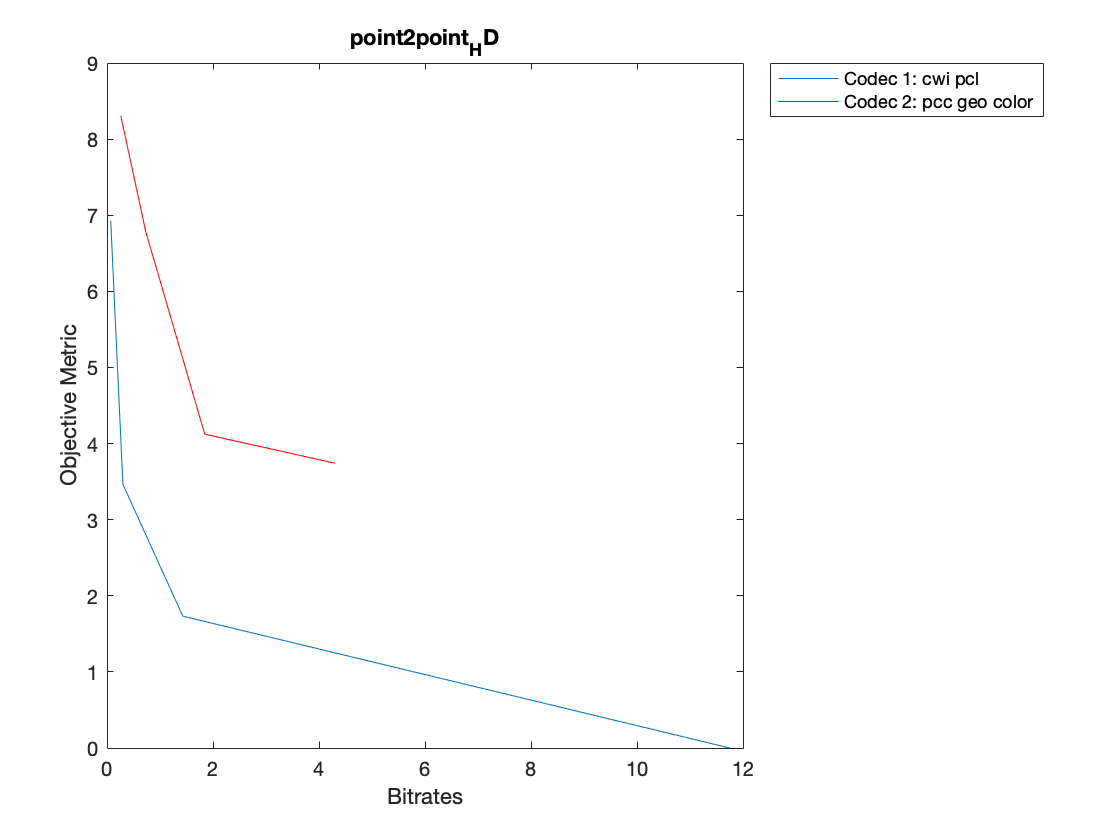
\includegraphics[width=\textwidth]{Figures/task2/longdress_p2p_hd.png}
    \subcaption{Point to point metric using Hausdorff distance.}
    \end{subfigure}

    \begin{subfigure}[b]{0.65\textwidth}
    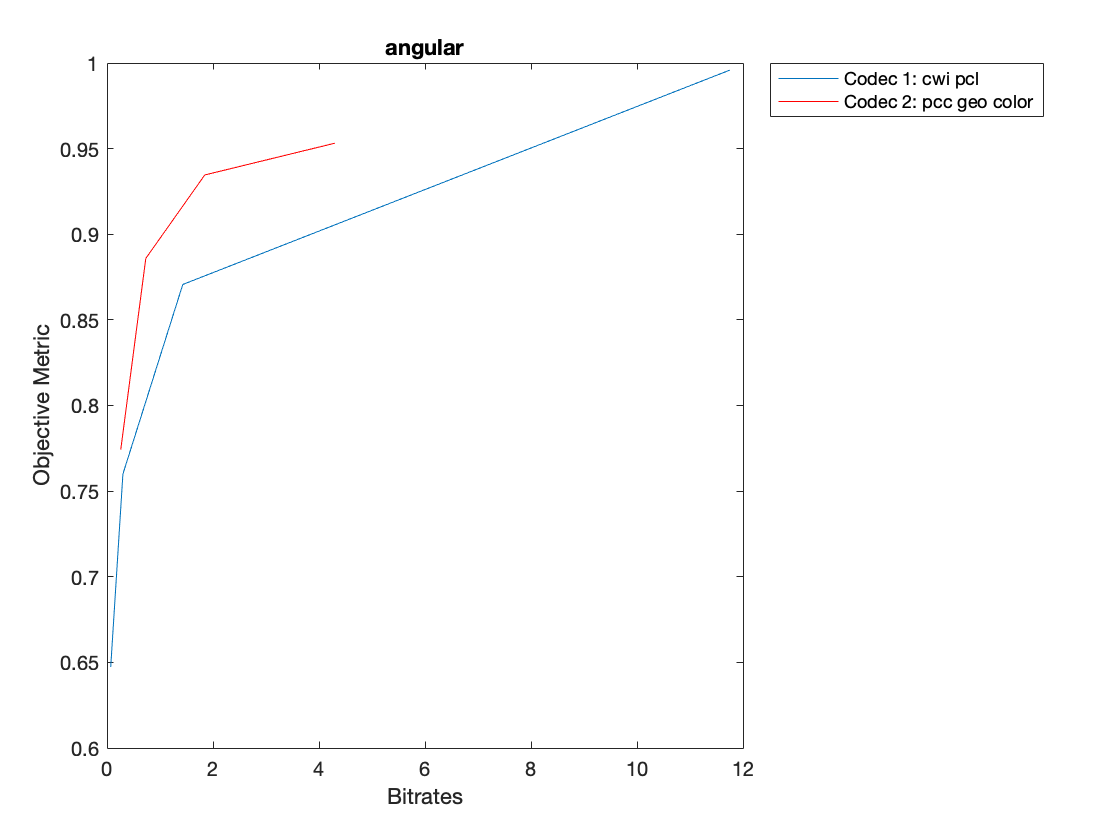
\includegraphics[width=\textwidth]{Figures/task2/longdress_angular.png}
    \subcaption{Plane to plane metric, computing angular similarity.}
    \end{subfigure}
\end{figure}

\begin{figure}
 \ContinuedFloat
    
    \begin{subfigure}[b]{0.65\textwidth}
    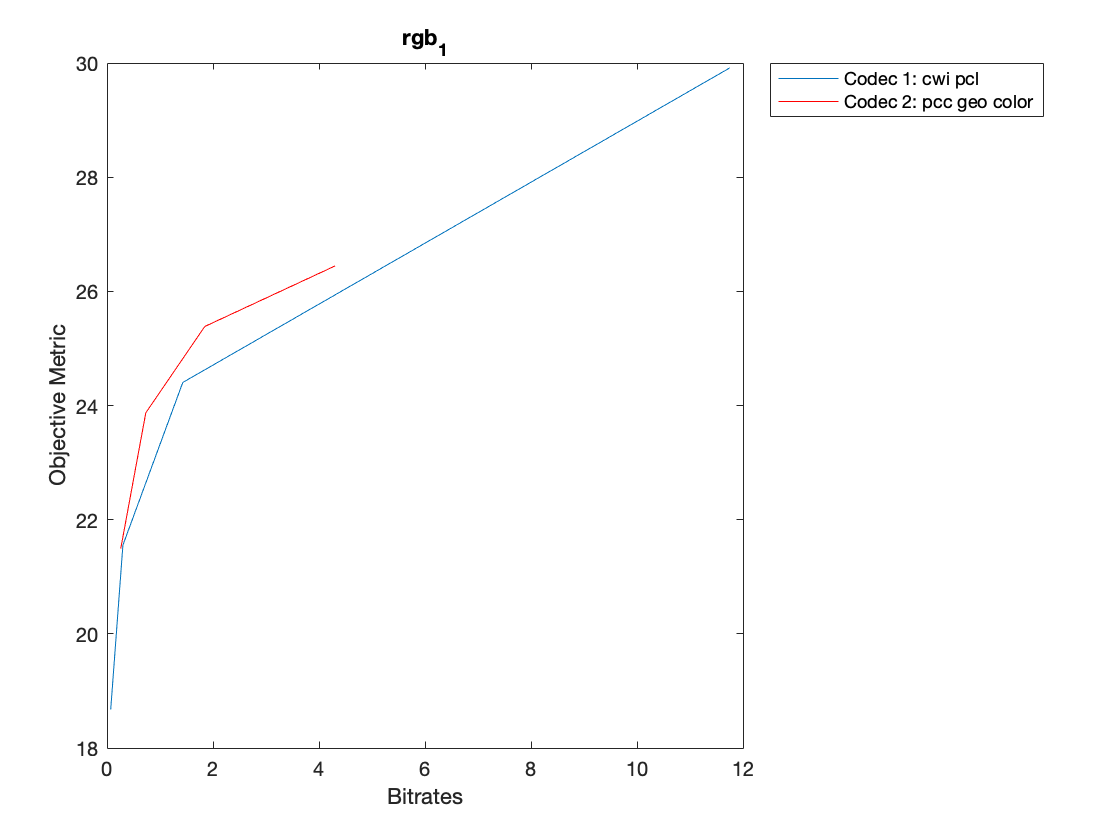
\includegraphics[width=\textwidth]{Figures/task2/longdress_rgb1.png}
    \subcaption{Symmetric color-PSNR, RGB space using eq. 14.}
    \end{subfigure}

    \begin{subfigure}[b]{0.65\textwidth}
    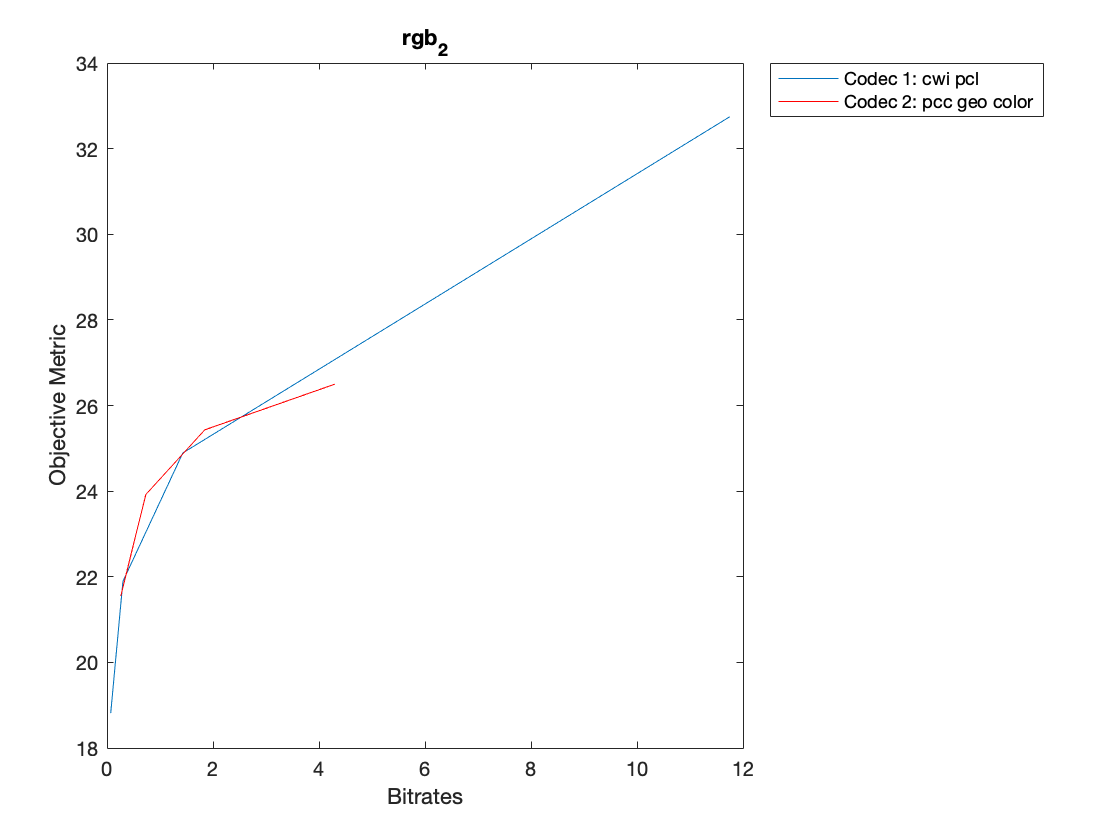
\includegraphics[width=\textwidth]{Figures/task2/longdress_rgb2.png}
    \subcaption{Symmetric color-PSNR, RGB space using eq. 15.}
    \end{subfigure}
    
    \begin{subfigure}[b]{0.65\textwidth}
    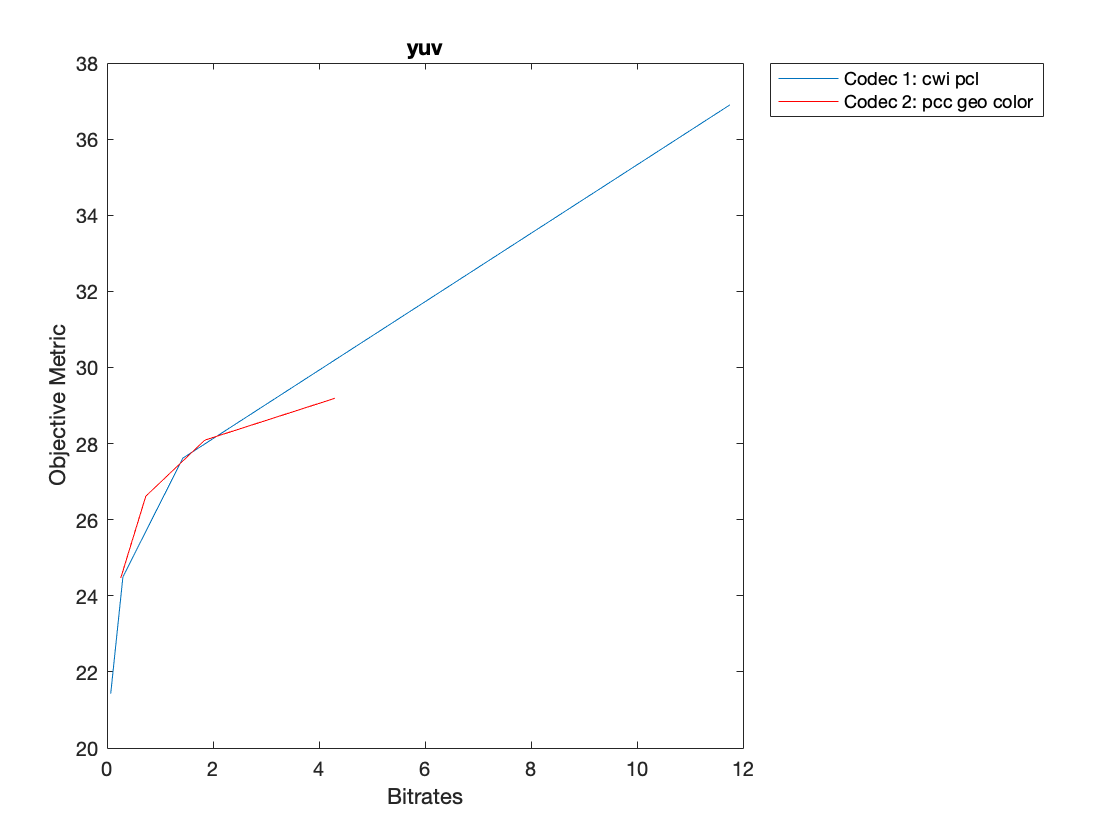
\includegraphics[width=\textwidth]{Figures/task2/longdress_yuv.png}
    \subcaption{Symmetric color-PSNR, YUV space.}
    \end{subfigure}
    \caption{Objective quality assessment on \textsf{longdress} point cloud.}
    \label{fig:obj_longdress}
\end{figure}

% Phil
\begin{figure}
    \centering
    \begin{subfigure}[b]{0.65\textwidth}
    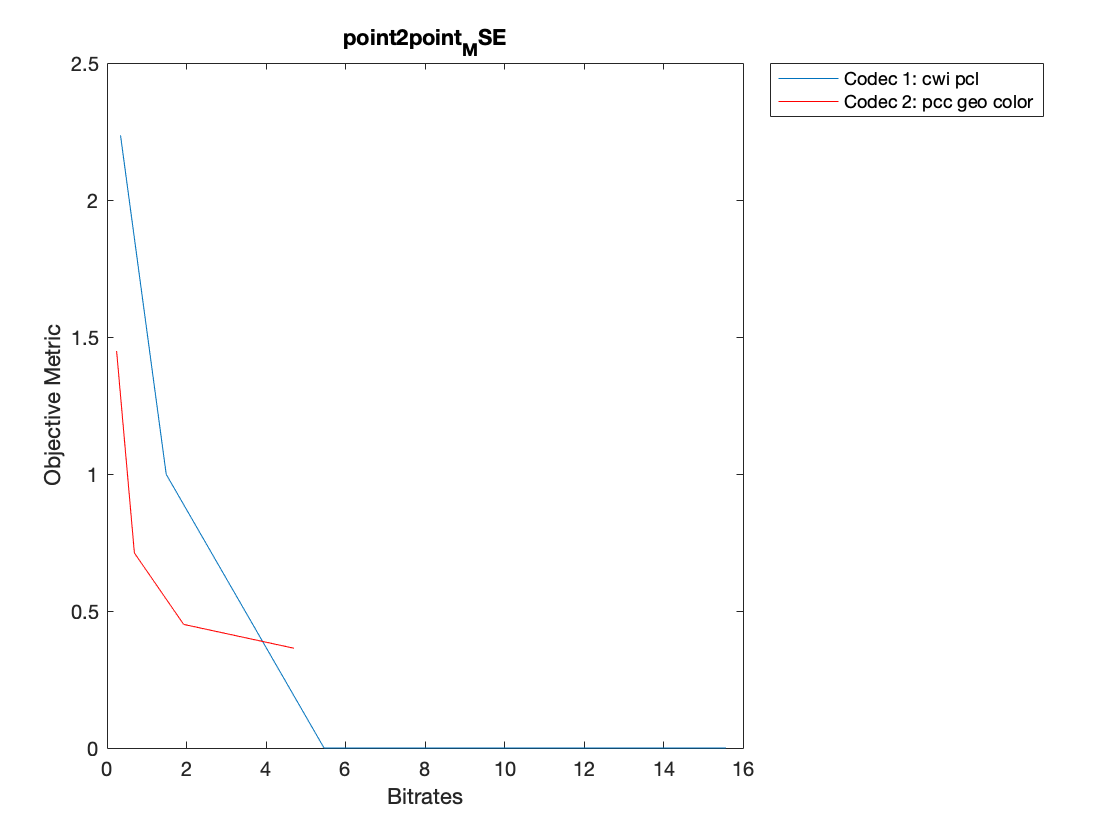
\includegraphics[width=\textwidth]{Figures/task2/phil_p2p_mse.png}
    \subcaption{Point to point metric using MSE.}
    \end{subfigure}

    \begin{subfigure}[b]{0.65\textwidth}
    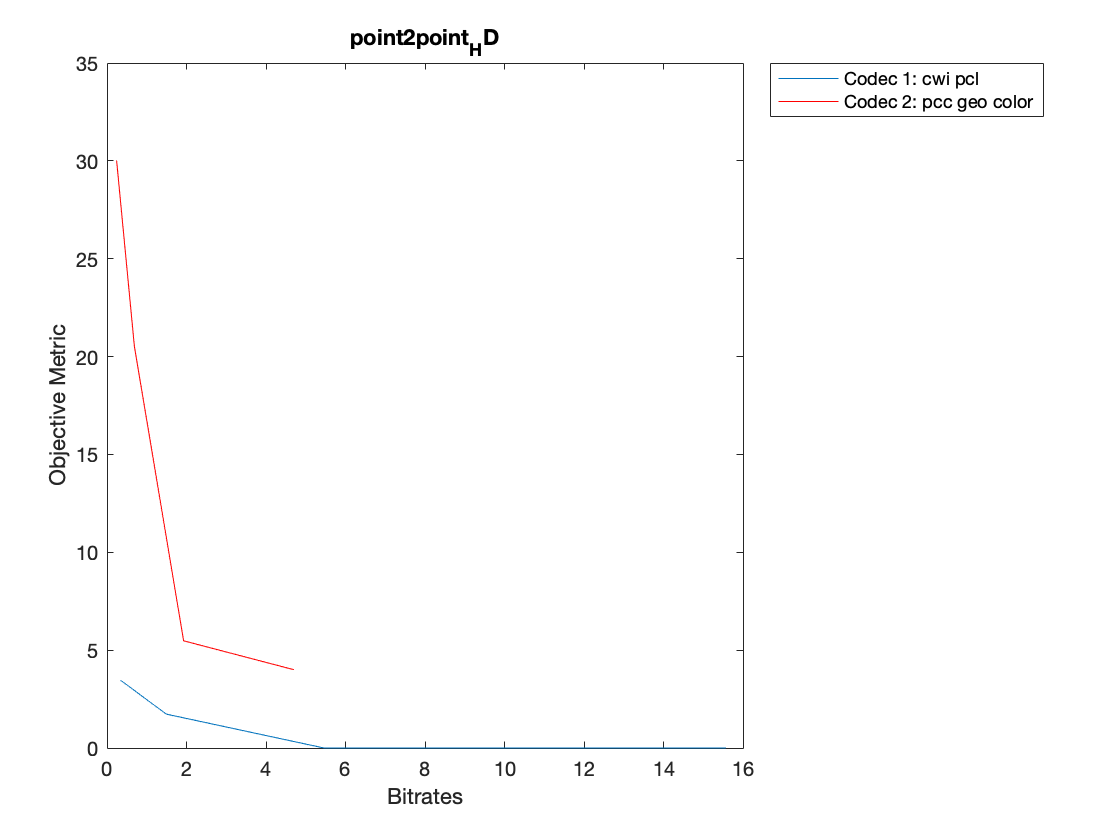
\includegraphics[width=\textwidth]{Figures/task2/phil_p2p_hd.png}
    \subcaption{Point to point metric using Hausdorff distance.}
    \end{subfigure}

    \begin{subfigure}[b]{0.65\textwidth}
    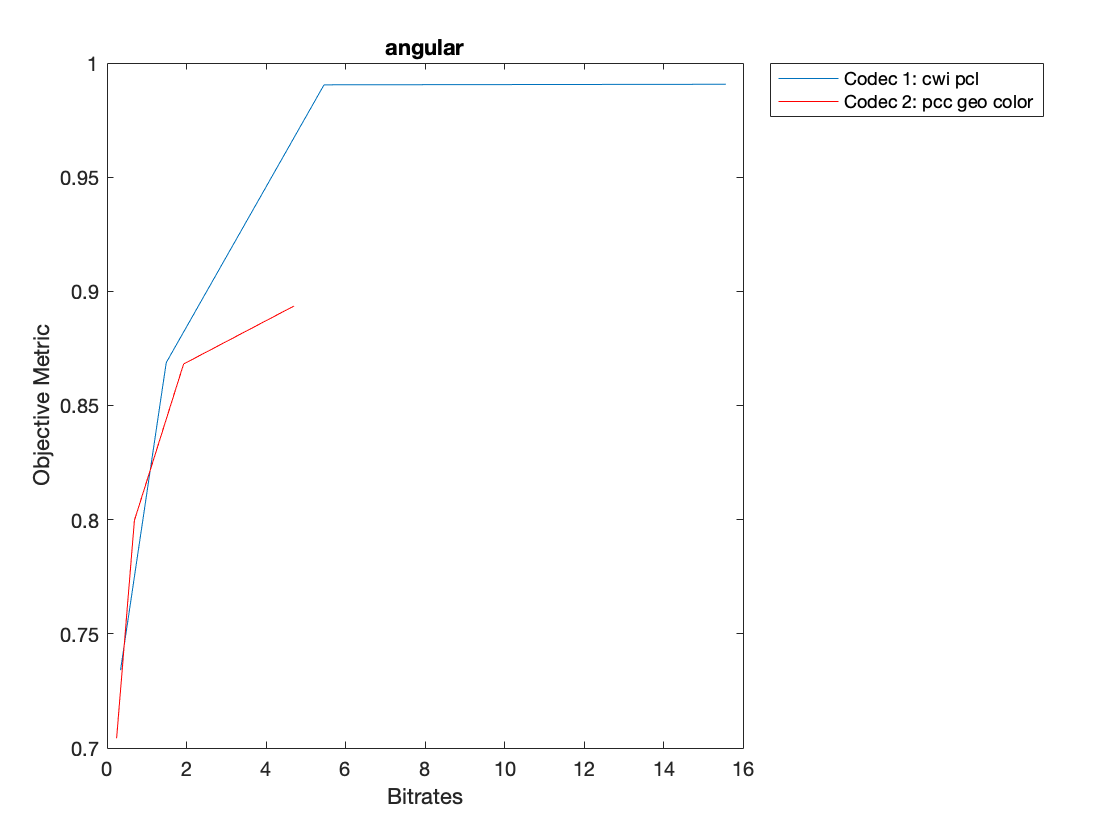
\includegraphics[width=\textwidth]{Figures/task2/phil_angular.png}
    \subcaption{Plane to plane metric, computing angular similarity.}
    \end{subfigure}

\end{figure}
\begin{figure}
 \ContinuedFloat

    \begin{subfigure}[b]{0.65\textwidth}
    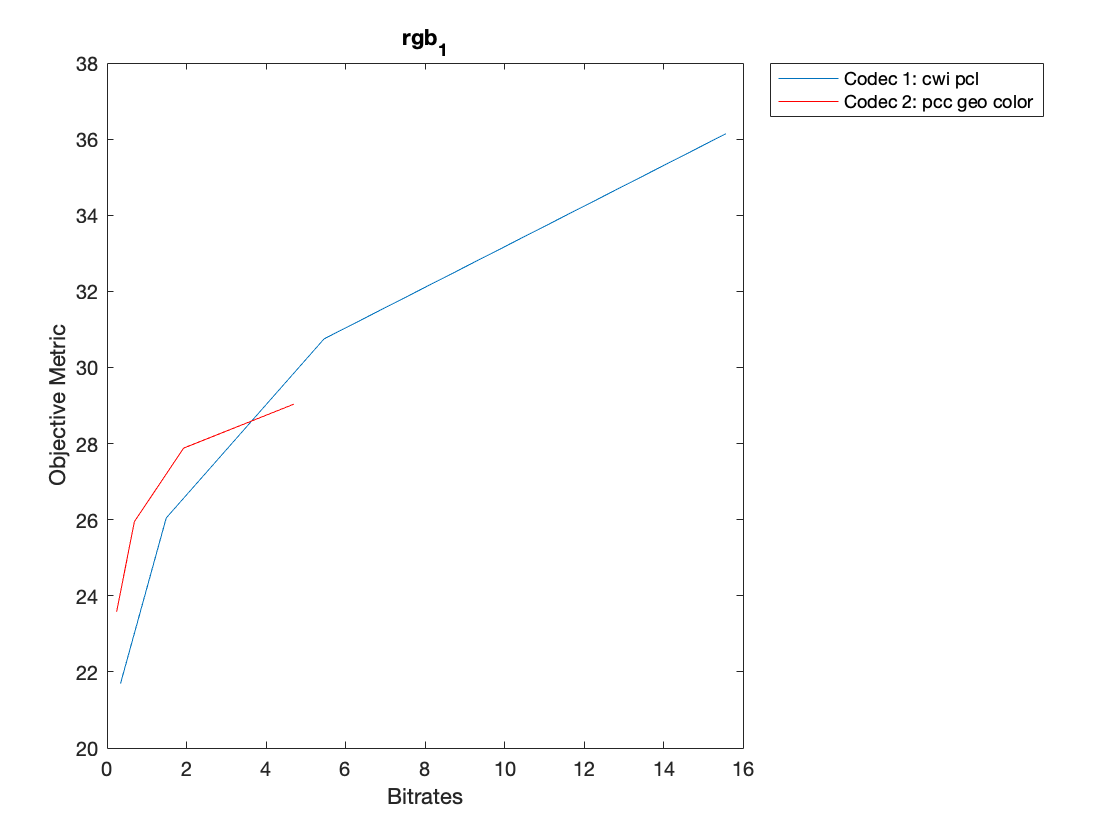
\includegraphics[width=\textwidth]{Figures/task2/phil_rgb1.png}
    \subcaption{Symmetric color-PSNR, RGB space using eq. 14.}
    \end{subfigure}
    
    \begin{subfigure}[b]{0.65\textwidth}
    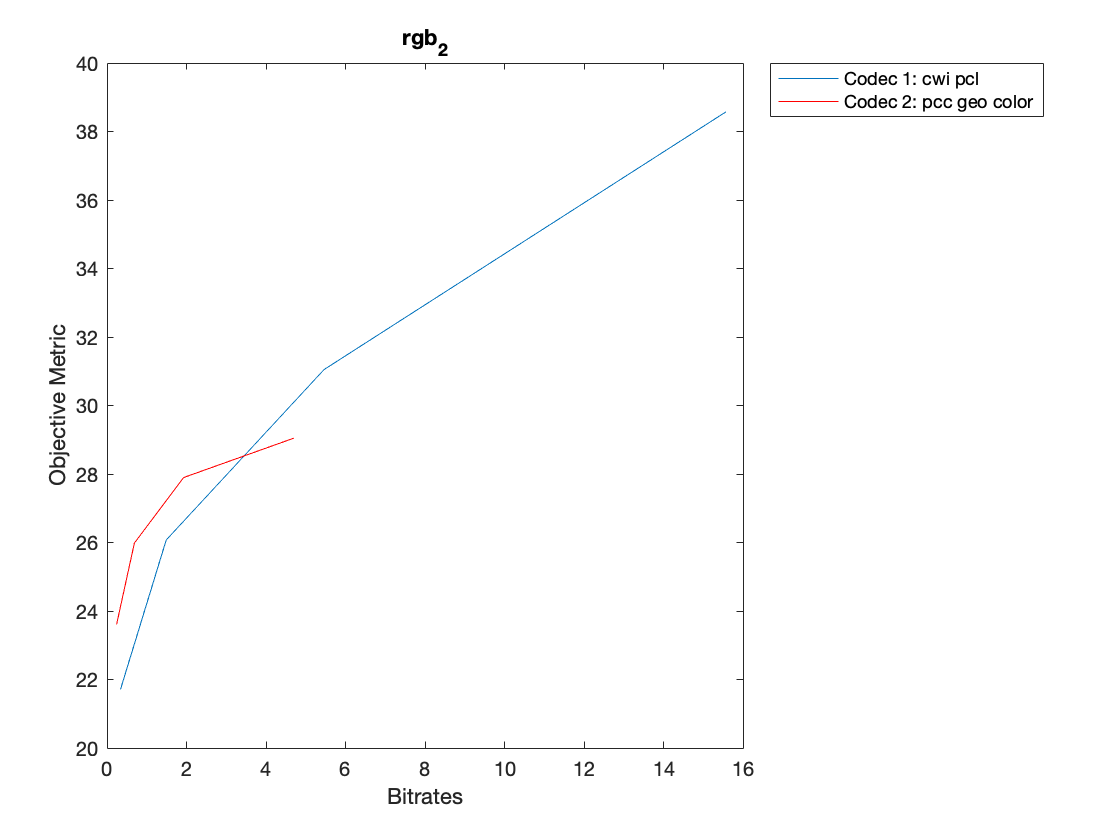
\includegraphics[width=\textwidth]{Figures/task2/phil_rgb2.png}
    \subcaption{Symmetric color-PSNR, RGB space using eq. 15.}
    \end{subfigure}
    
    \begin{subfigure}[b]{0.65\textwidth}
    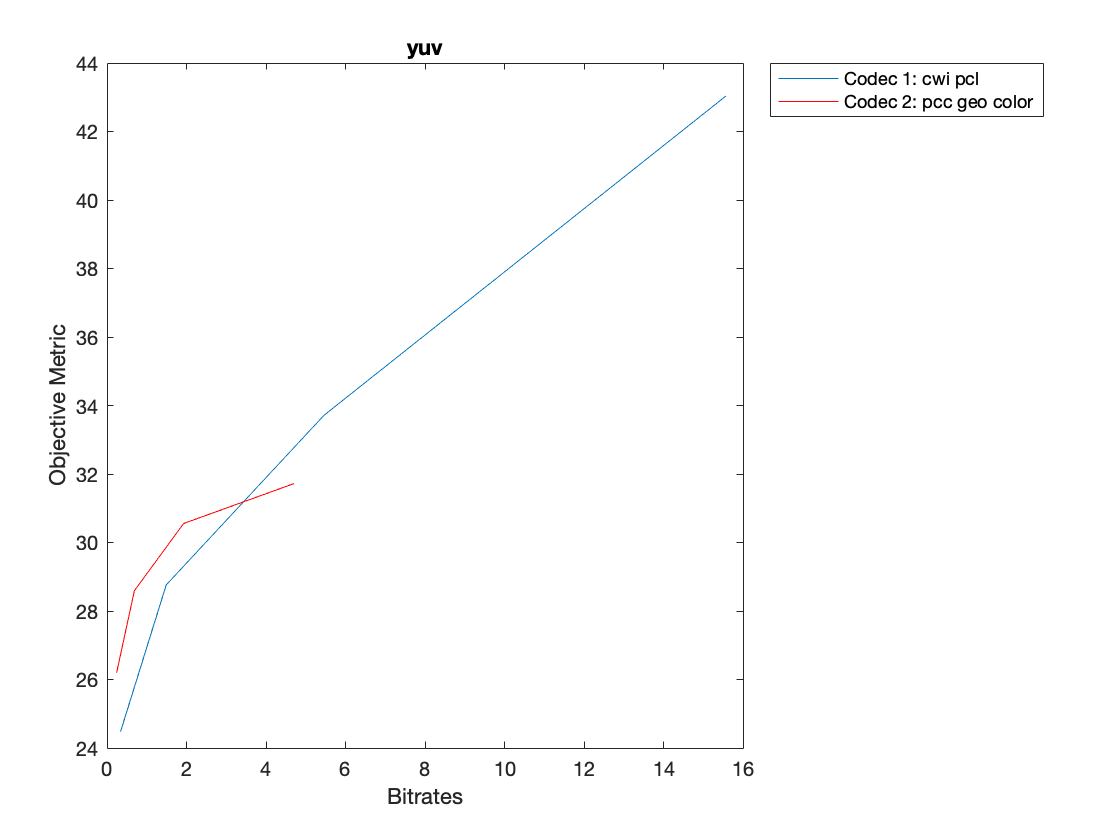
\includegraphics[width=\textwidth]{Figures/task2/phil_yuv.png}
    \subcaption{Symmetric color-PSNR, YUV space.}
    \end{subfigure}
    \caption{Objective quality assessment on \textsf{phil} point cloud.}
    \label{fig:obj_phil}
\end{figure}

% Rhetorician
\begin{figure}
    \centering
    \begin{subfigure}[b]{0.65\textwidth}
    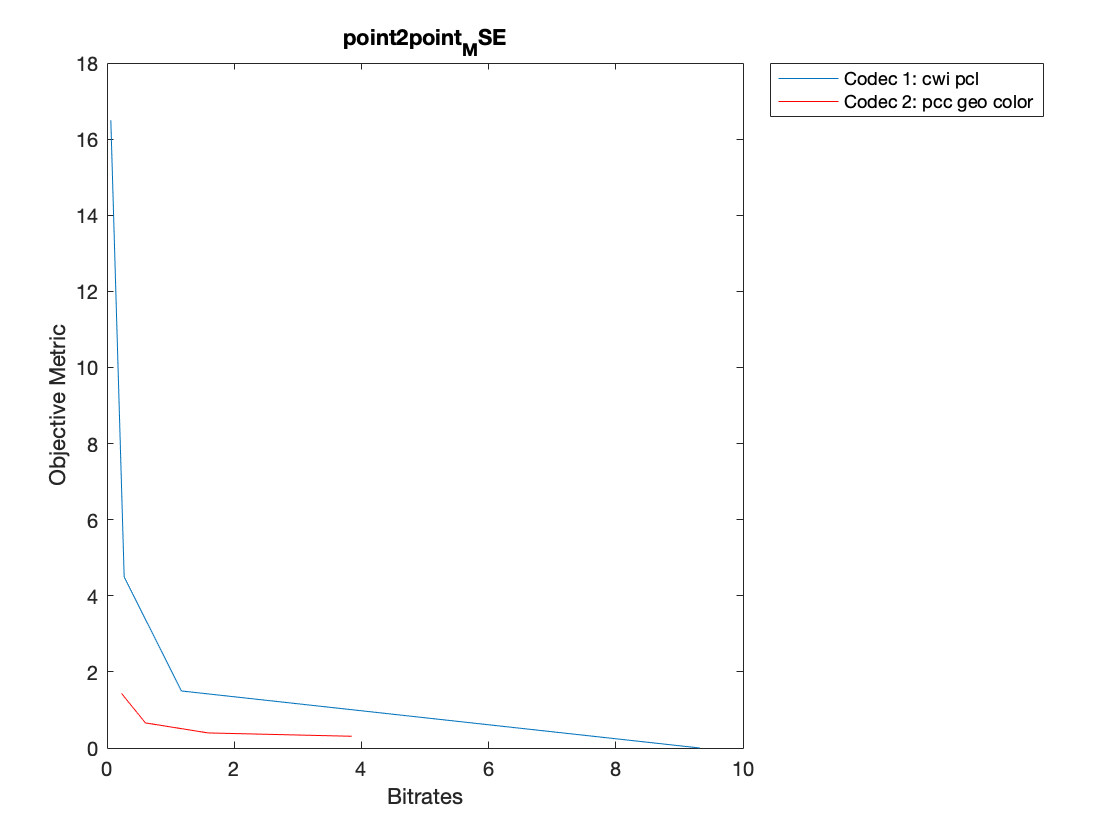
\includegraphics[width=\textwidth]{Figures/task2/rhetorician_p2p_mse.png}
    \subcaption{Point to point metric using MSE.}
    \end{subfigure}

    \begin{subfigure}[b]{0.65\textwidth}
    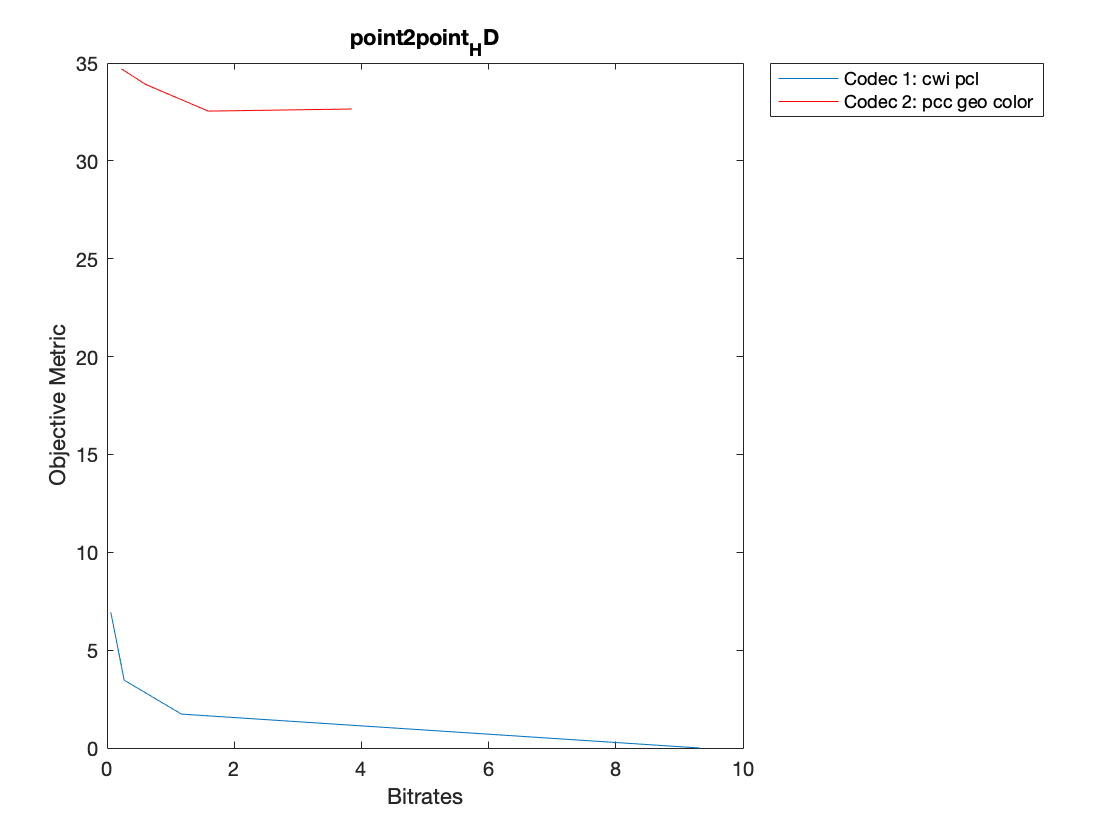
\includegraphics[width=\textwidth]{Figures/task2/rhetorician_p2p_hd.png}
    \subcaption{Point to point metric using Hausdorff distance.}
    \end{subfigure}

    \begin{subfigure}[b]{0.65\textwidth}
    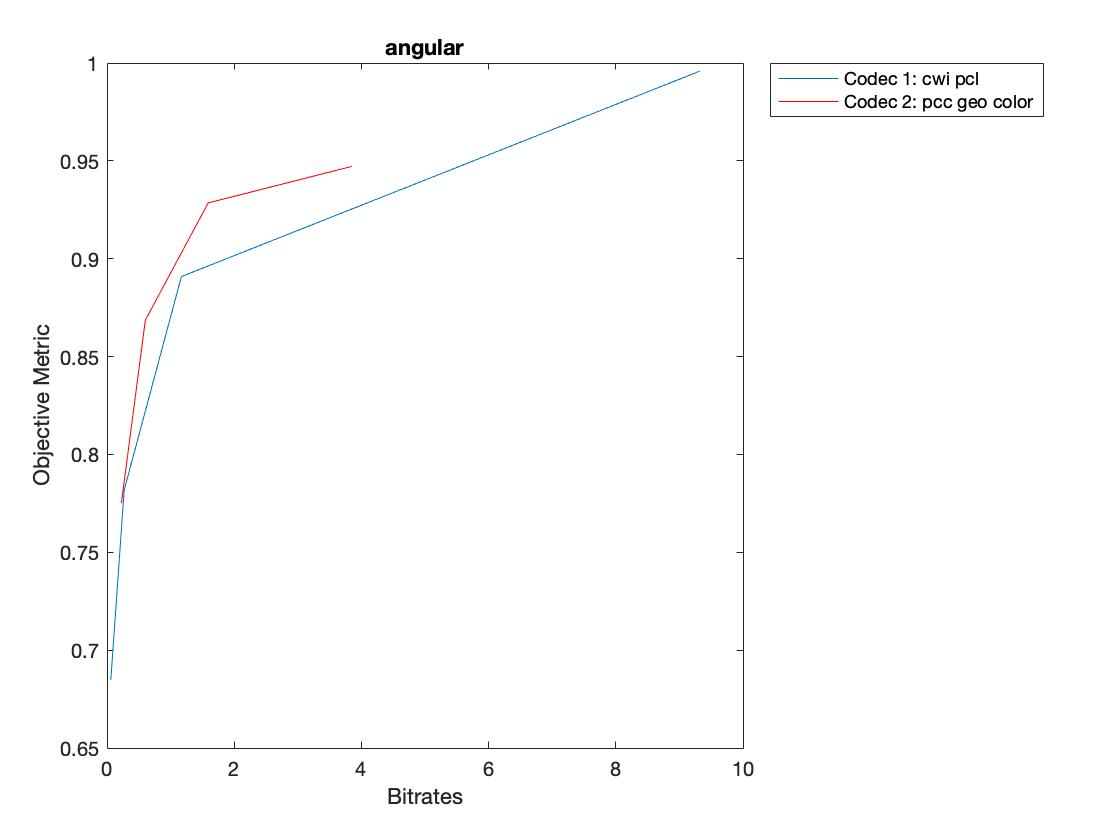
\includegraphics[width=\textwidth]{Figures/task2/rhetorician_angular.png}
    \subcaption{Plane to plane metric, computing angular similarity.}
    \end{subfigure}
\end{figure}

\begin{figure}
 \ContinuedFloat
    \begin{subfigure}[b]{0.65\textwidth}
    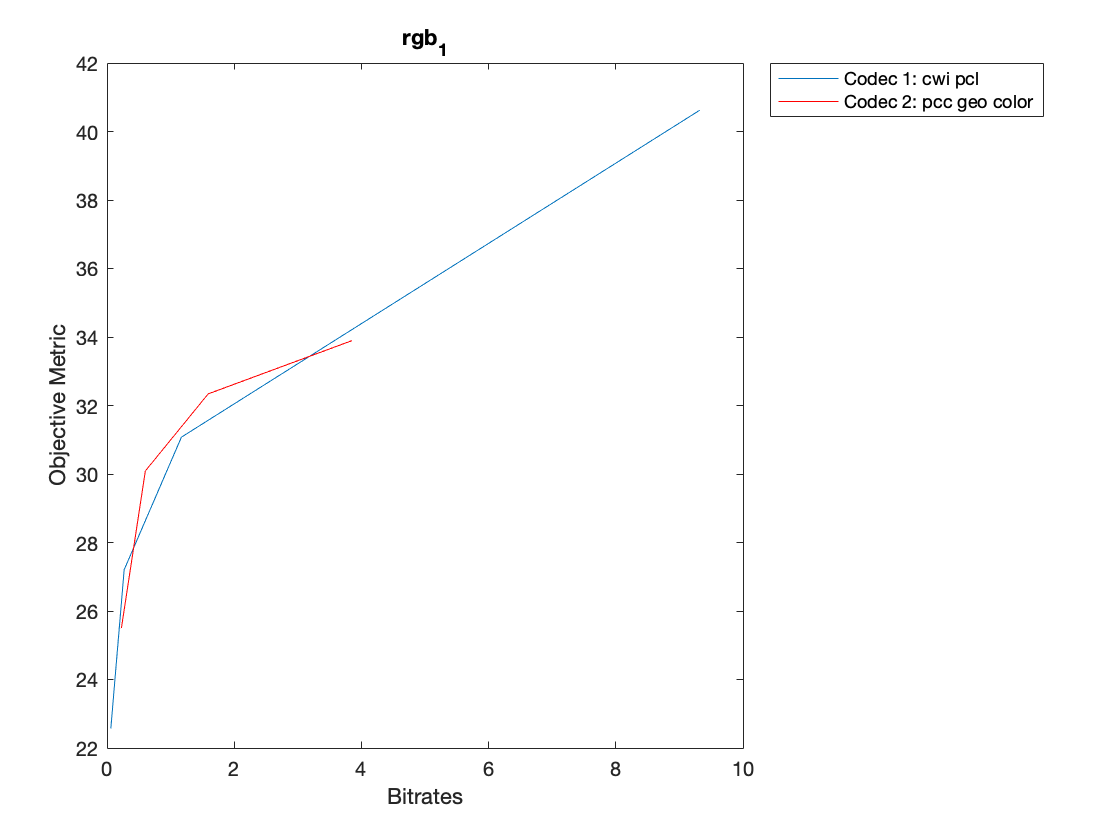
\includegraphics[width=\textwidth]{Figures/task2/rhetorician_rgb1.png}
    \subcaption{Symmetric color-PSNR, RGB space using eq. 14.}
    \end{subfigure}

    \begin{subfigure}[b]{0.65\textwidth}
    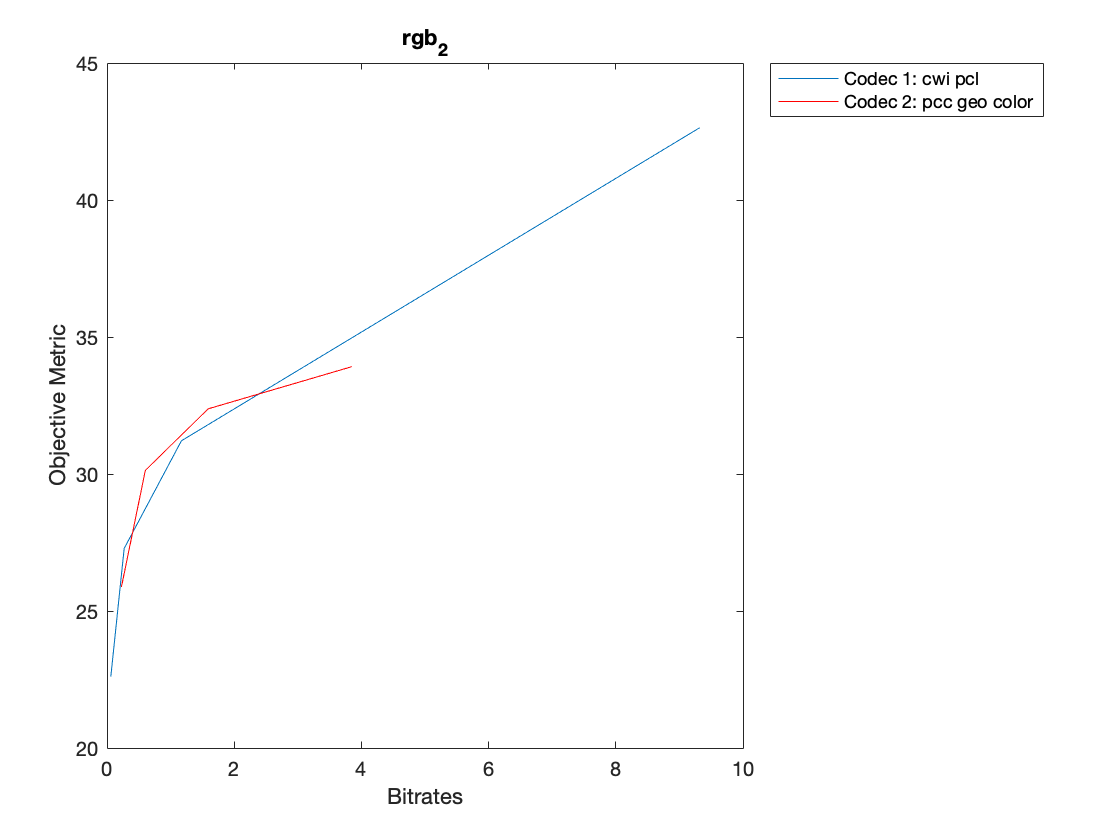
\includegraphics[width=\textwidth]{Figures/task2/rhetorician_rgb2.png}
    \subcaption{Symmetric color-PSNR, RGB space using eq. 15.}
    \end{subfigure}
    
    \begin{subfigure}[b]{0.65\textwidth}
    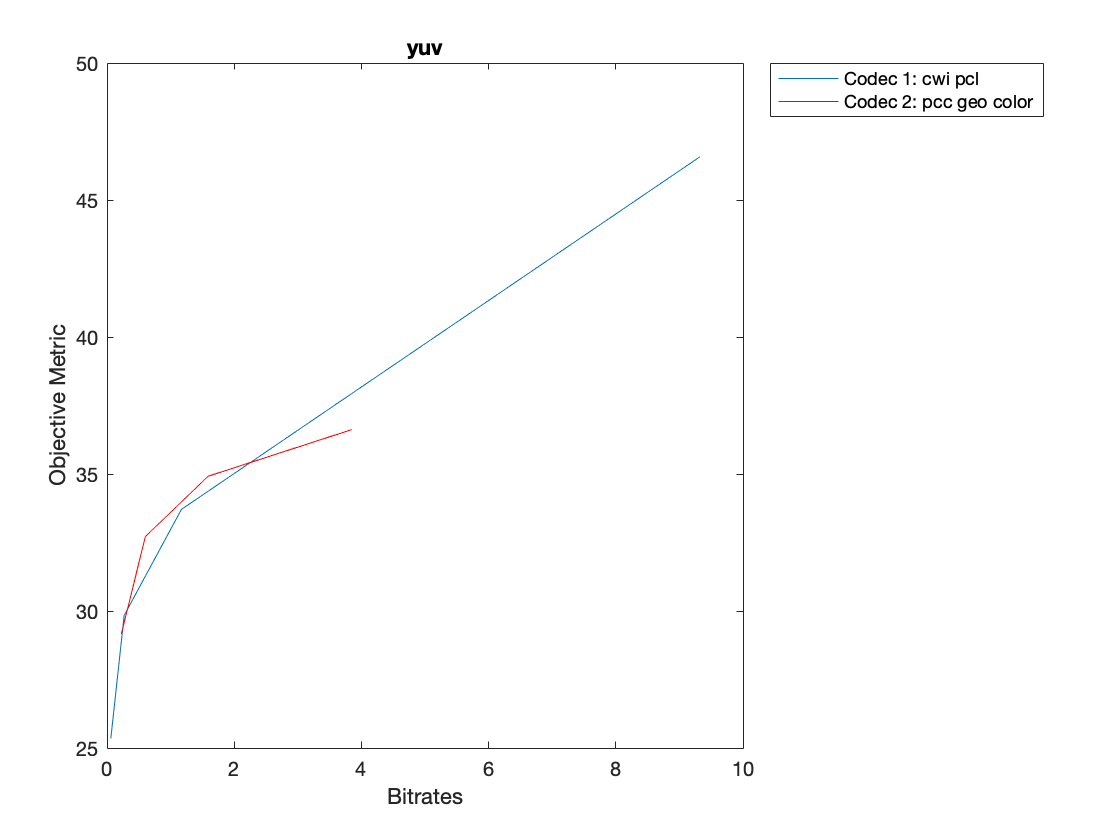
\includegraphics[width=\textwidth]{Figures/task2/rhetorician_yuv.png}
    \subcaption{Symmetric color-PSNR, YUV space.}
    \end{subfigure}
    \caption{Objective quality assessment on \textsf{phil} point cloud.}
    \label{fig:obj_rhetorician}
\end{figure}


\section{Benchmarking of Objective Quality Metrics}
In this exercise, we compare the correlation between the DMOS and the objective results using Pearson's and Spearman's correlation coefficient as well as the RMSE.
Additionally, we use linear and cubic fitting to fit the objective results to the DMOS and also look at the correlation for the fitted results. Table \ref{tab:1} reports the respected coefficients for each metric. Furthermore, Figure \ref{fig:p2p_mse_fitted} to \ref{fig:yuv_fitted} plot the DMOS against the objective values in their original setting, linearly fitted and cubicly fitted. \\

If we have a negative correlation coefficient, this means that the two variables for which we compute the correlation coefficient develop in opposite direction (i.e. DMOS increases while error decreases or vise versa). The larger the coefficient, the stronger the correlation. Pearson compares the linear relation between two variables, while Spearman looks at the monotonic relation between two variables. RMSE is simply a measure for capturing the difference between two variables. \\

With this knowledge, we can make the following observations with Table \ref{tab:1}: It clearly indicates is that if the objective results are fitted cubicly, the Pearson and the Spearman coefficient increase, while the RMSE decreases for all metrics. Thus, one can say that the cubicly fitted objective results better describe the relation between the subjective and the objective data independent of the metric. For the point 2 point metrics (using MSE and Hausdorff distance), the correlation coefficients experience a sign change when fitting the data cubicly and linearly. Thus, those metrics do not seem to robustly representation between the subjective and the objective scores. The correlation coefficients of the angular similarity metric remains pretty constant through the fitting and achieves the highest values across all metrics. For the color metrics, we also achieve quite robust values over the fitting phase. However, in contrast to the angular similarity, the Pearson and Spearman coefficients remain smaller. Thus, it is reasonable to say the angular similarity metric seems to be an objective measure describing subjective visual quality the best. 


\begin{table}[t]
\caption{Correlation coefficients between DMOS and the objective results for different metrics using Pearson's (P) and Spearman's (S) correlation coefficient as well as RMSE for the original objective values, linearly (l) and cubicly (c) fitted data.}
\label{tab:1}
\begin{tabular}{c | c c c c c c c c c}
metric & P & S & RMSE & P (l) & S (l) & RMSE(l) & P (c) & S (c) & RMSE (c) \\
\hline
p2p(MSE) & -0.81 & -0.9 &	31.70 &	0.81 &	0.9	& 3.70 & 0.93 &	0.9 &	2.24 \\
p2p (HD) & -0.07 & -0.44 & 69.69 & 0.08 &	0.44 &	6.27 &	0.65 &	0.6 &	4.8 \\
angular & 0.93 & 0.91 &	17.1 &	0.93 &	0.91 &	2.36 &	0.93 &	0.91 &	2.31 \\
rgb1 & 0.78 &	0.85 &	132.76 & 0.78 &	0.85 &	3.97 &	0.86 &	0.85 &	3.26 \\
rgb2 & 0.76 &	0.86 &	135.48 & 0.76 &	0.86 &	4.08 &	0.85 &	0.86 &	3.27 \\
yuv & 0.75 &	0.85 &	151.91 & 0.75 &	0.85 &	4.16 &	0.85 &	0.85 &	3.28
\end{tabular}
\end{table}


\begin{figure}
    
    \centering
   \begin{subfigure}[b]{0.65\textwidth}
   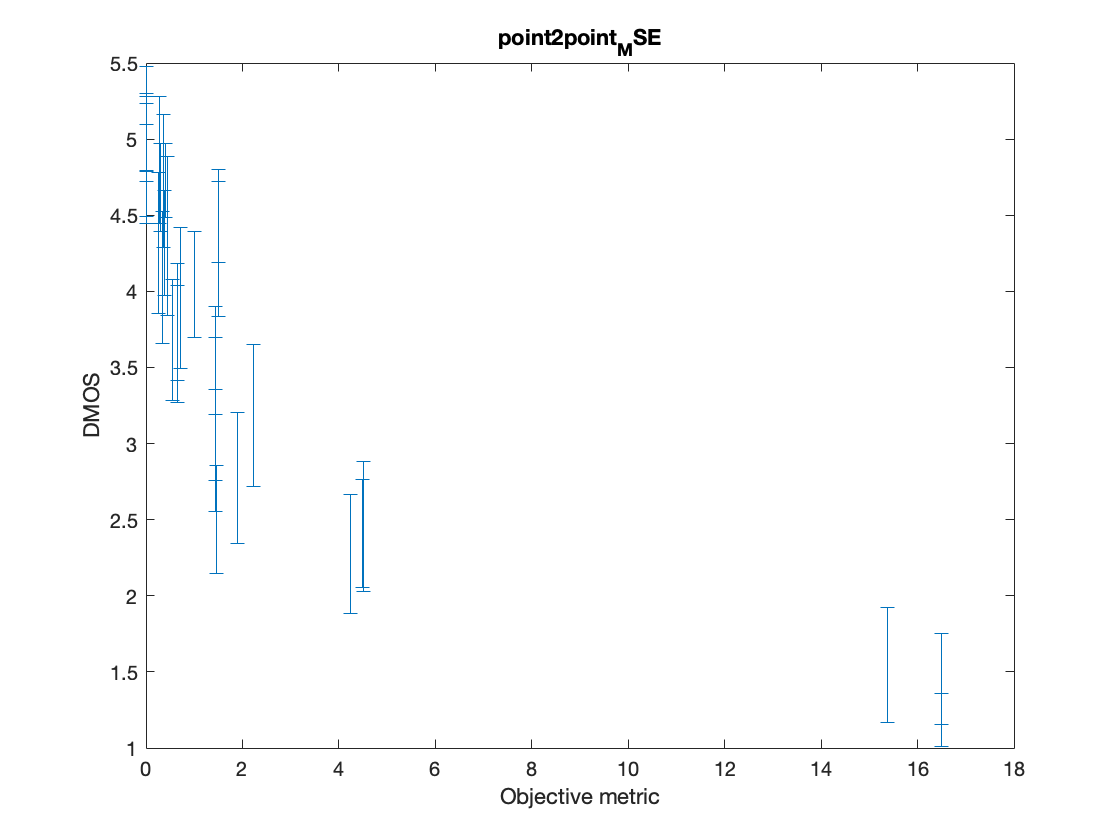
\includegraphics[width=\textwidth]{Figures/task3/p2p_mse.png}
   \end{subfigure}
   
   \begin{subfigure}[b]{0.65\textwidth}
   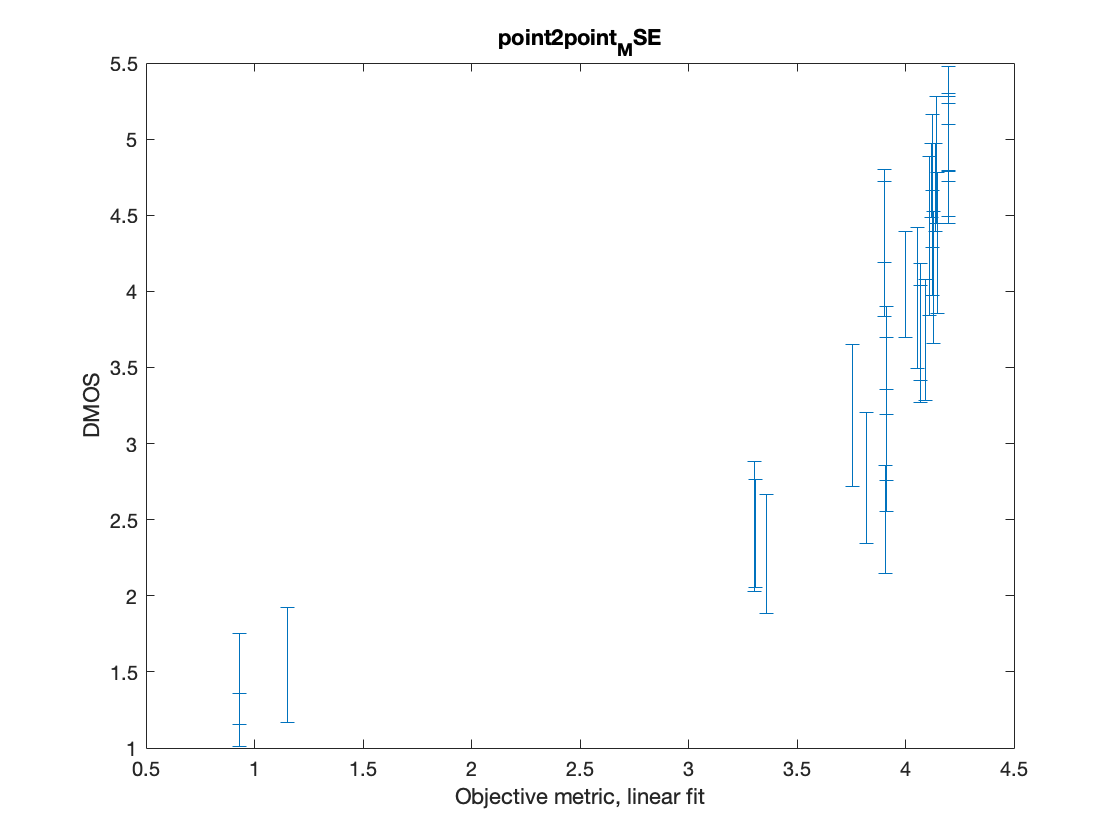
\includegraphics[width=\textwidth]{Figures/task3/p2p_mse_linear.png}
   \end{subfigure}
   
   \begin{subfigure}[b]{0.65\textwidth}
   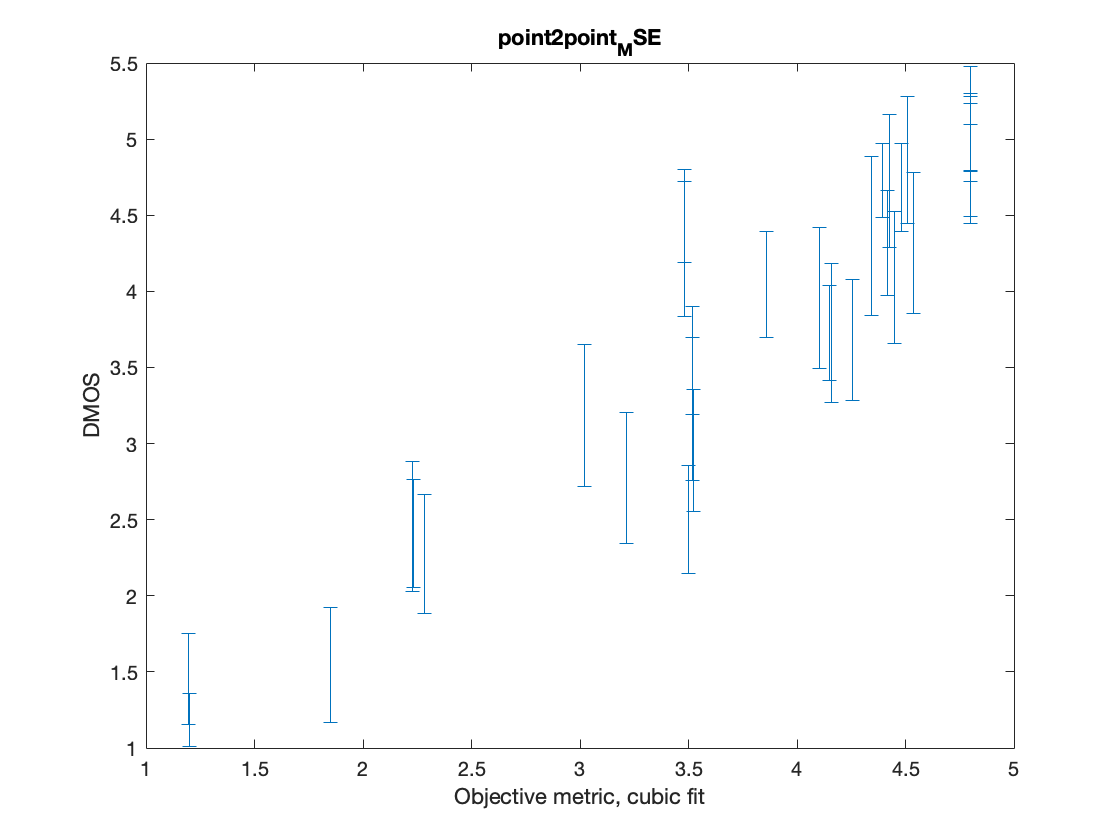
\includegraphics[width=\textwidth]{Figures/task3/p2p_mse_cubic.png}
   \end{subfigure}
    \caption{DMOS vs. point to point with MSE plain, linearly fitted, cubicly fitted.}
    \label{fig:p2p_mse_fitted}
\end{figure}

\begin{figure}
   
    \centering
   \begin{subfigure}[b]{0.65\textwidth}
   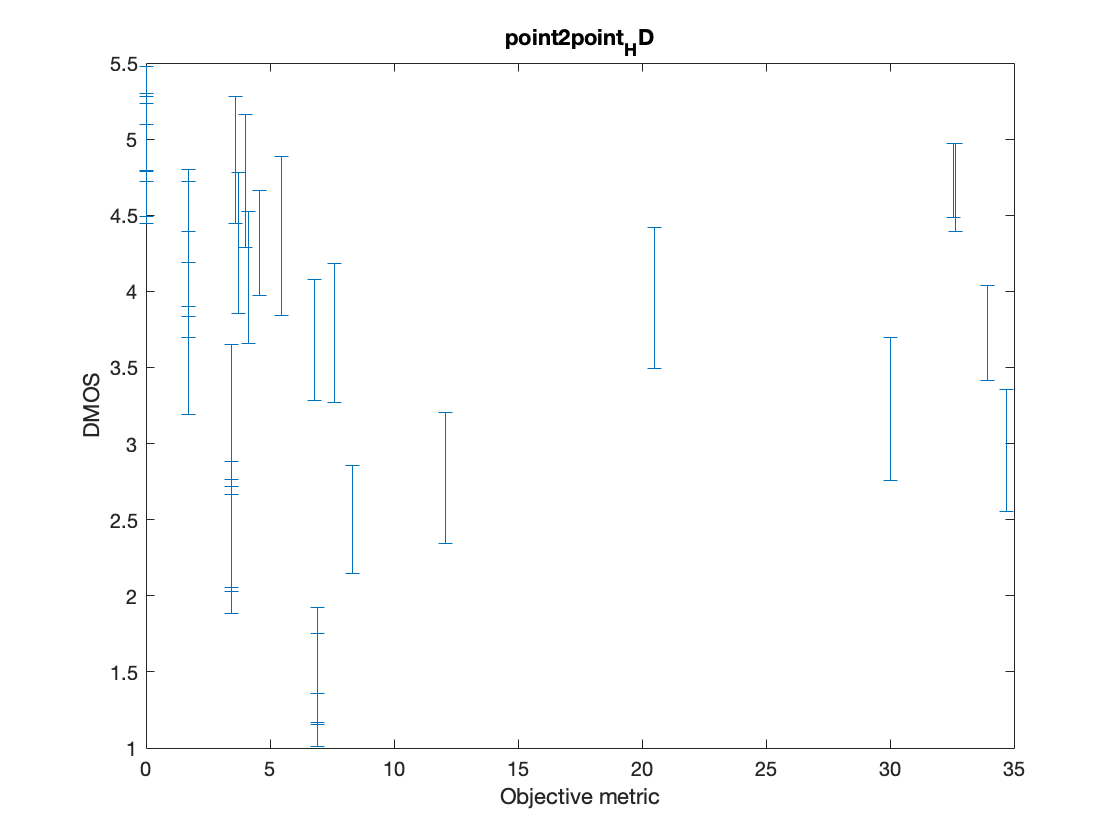
\includegraphics[width=\textwidth]{Figures/task3/p2p_hd.png}
   \end{subfigure}
   
   \begin{subfigure}[b]{0.65\textwidth}
   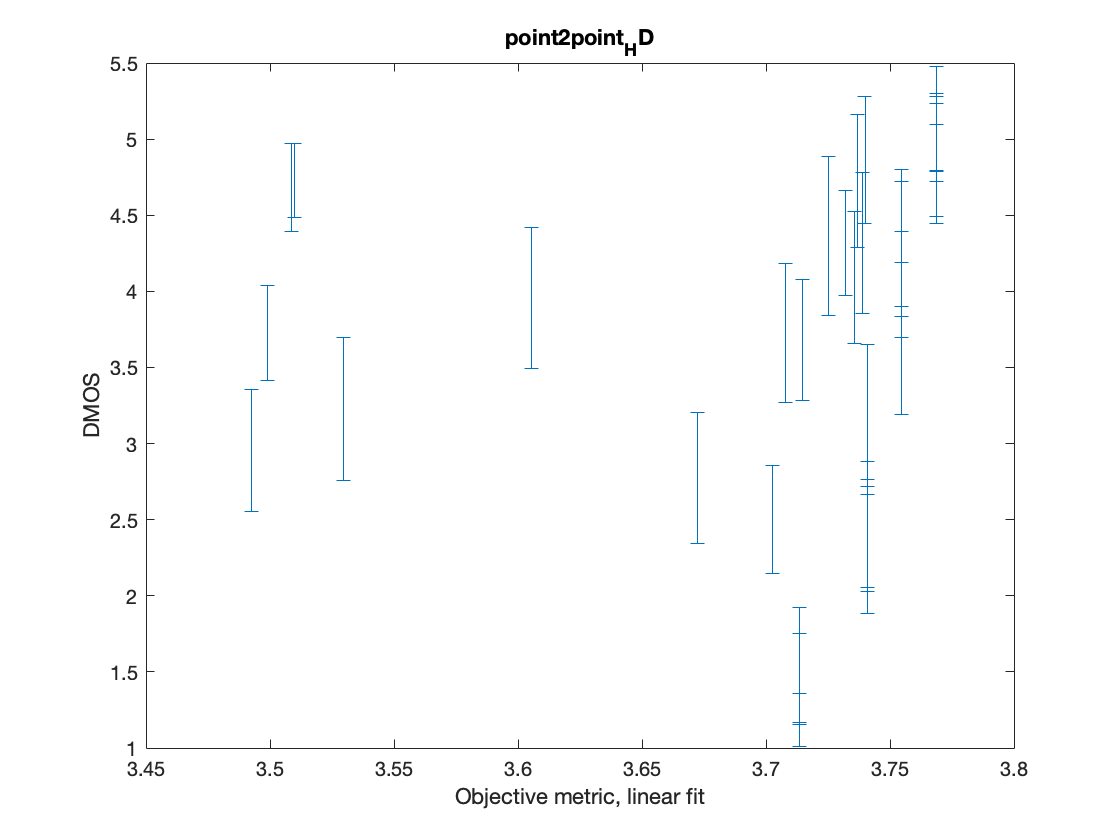
\includegraphics[width=\textwidth]{Figures/task3/p2p_hd_linear.png}
   \end{subfigure}
   
   \begin{subfigure}[b]{0.65\textwidth}
   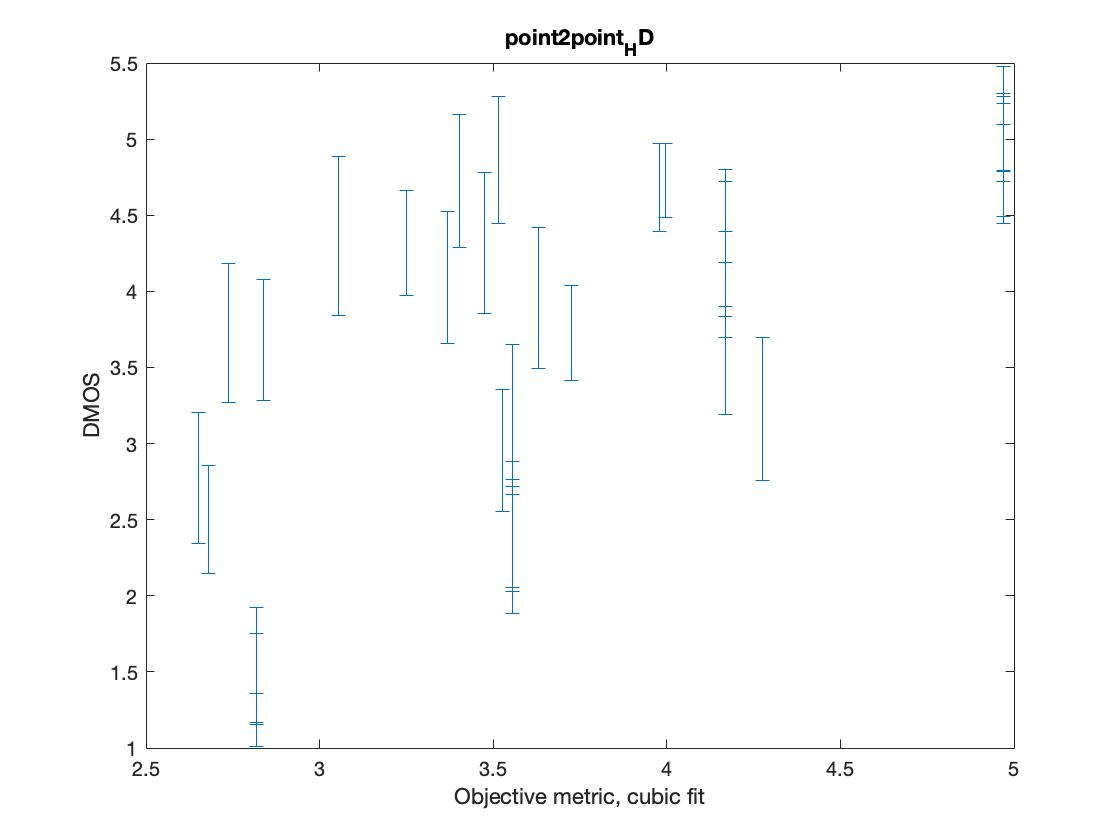
\includegraphics[width=\textwidth]{Figures/task3/p2p_hd_cubic.png}
   \end{subfigure}
    \caption{DMOS vs. point to point with Hausdorff distance plain, linearly fitted, cubicly fitted.}
    \label{fig:p2p_hd_fitted}
\end{figure}

\begin{figure}
    \centering
   \begin{subfigure}[b]{0.65\textwidth}
   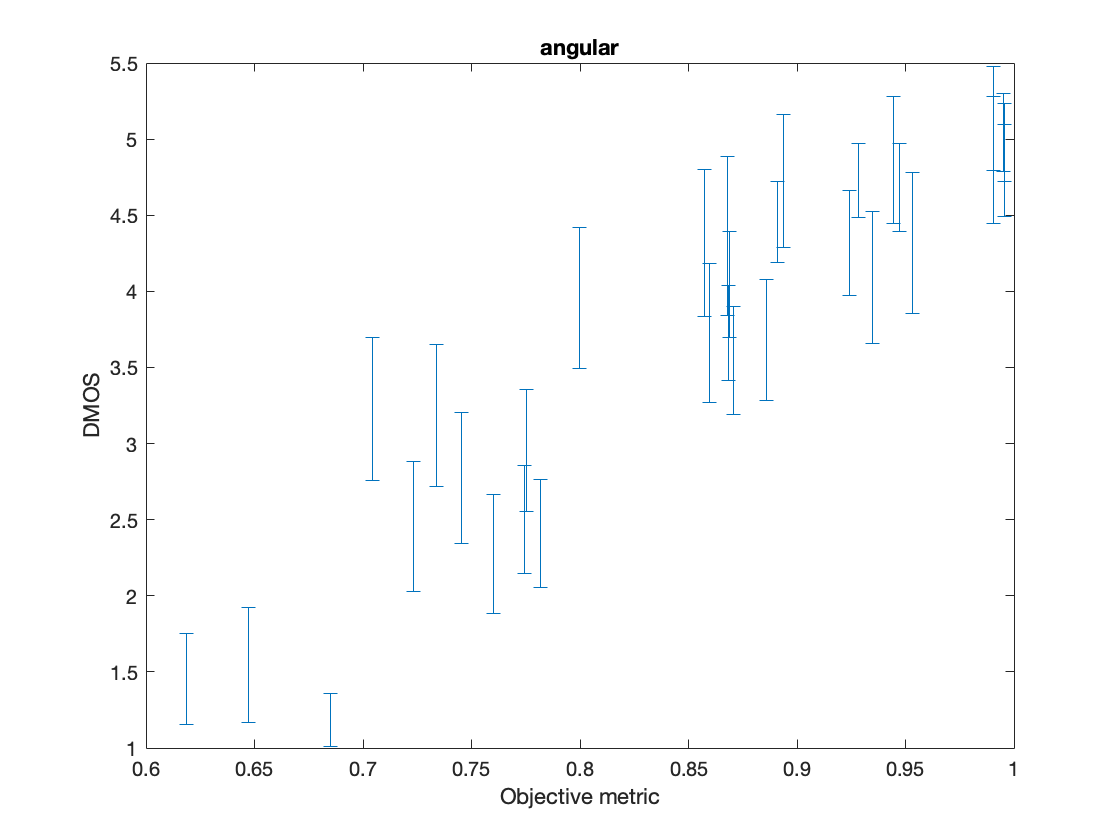
\includegraphics[width=\textwidth]{Figures/task3/angular.png}
   \end{subfigure}
   
   \begin{subfigure}[b]{0.65\textwidth}
   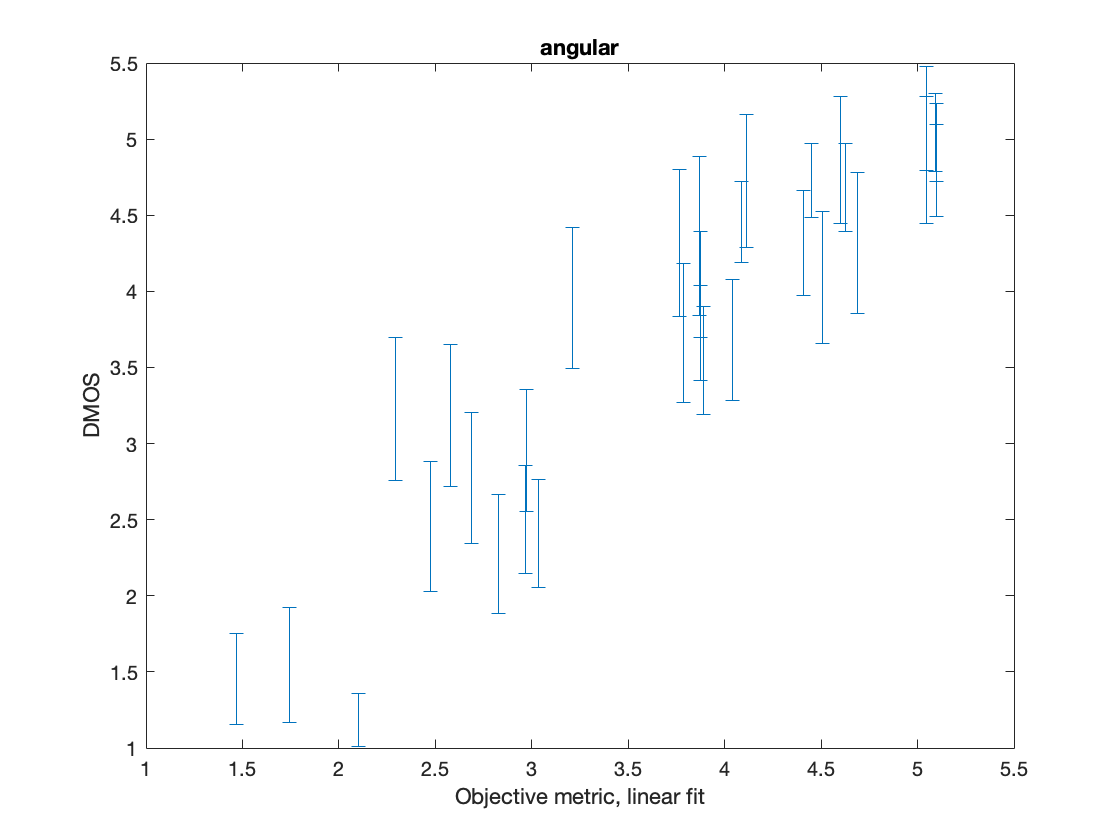
\includegraphics[width=\textwidth]{Figures/task3/angular_linear.png}
   \end{subfigure}
   
   \begin{subfigure}[b]{0.65\textwidth}
   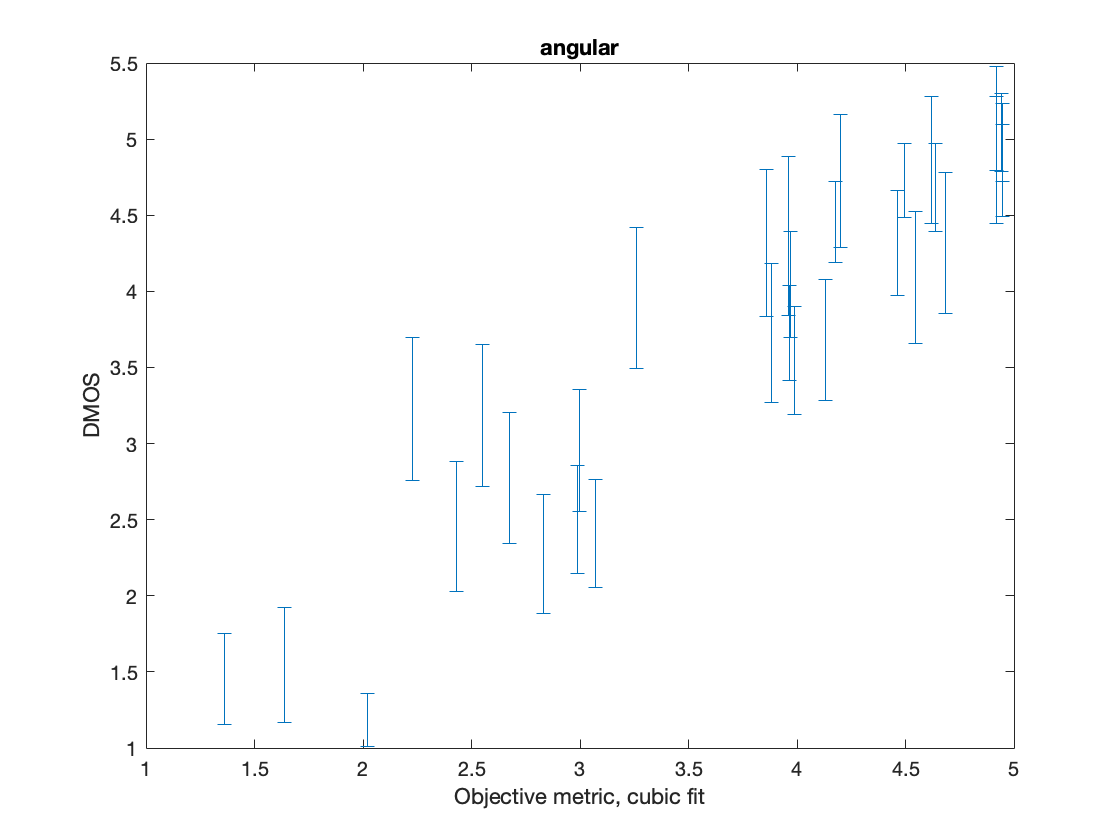
\includegraphics[width=\textwidth]{Figures/task3/angular_cubic.png}
   \end{subfigure}
    \caption{DMOS vs. plane to plane metric plain, linearly fitted, cubicly fitted.}
    \label{fig:angular_fitted}
\end{figure}

\begin{figure}
  
    \centering
   \begin{subfigure}[b]{0.65\textwidth}
   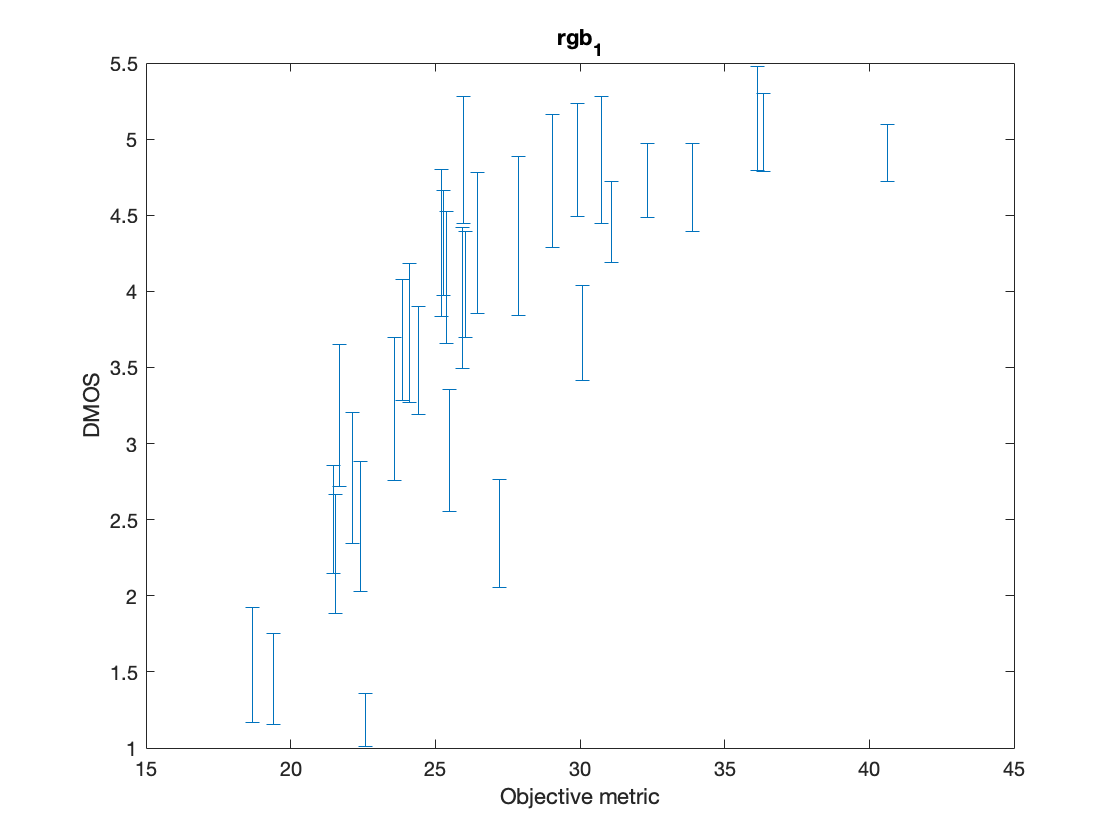
\includegraphics[width=\textwidth]{Figures/task3/rgb1.png}
   \end{subfigure}
   
   \begin{subfigure}[b]{0.65\textwidth}
   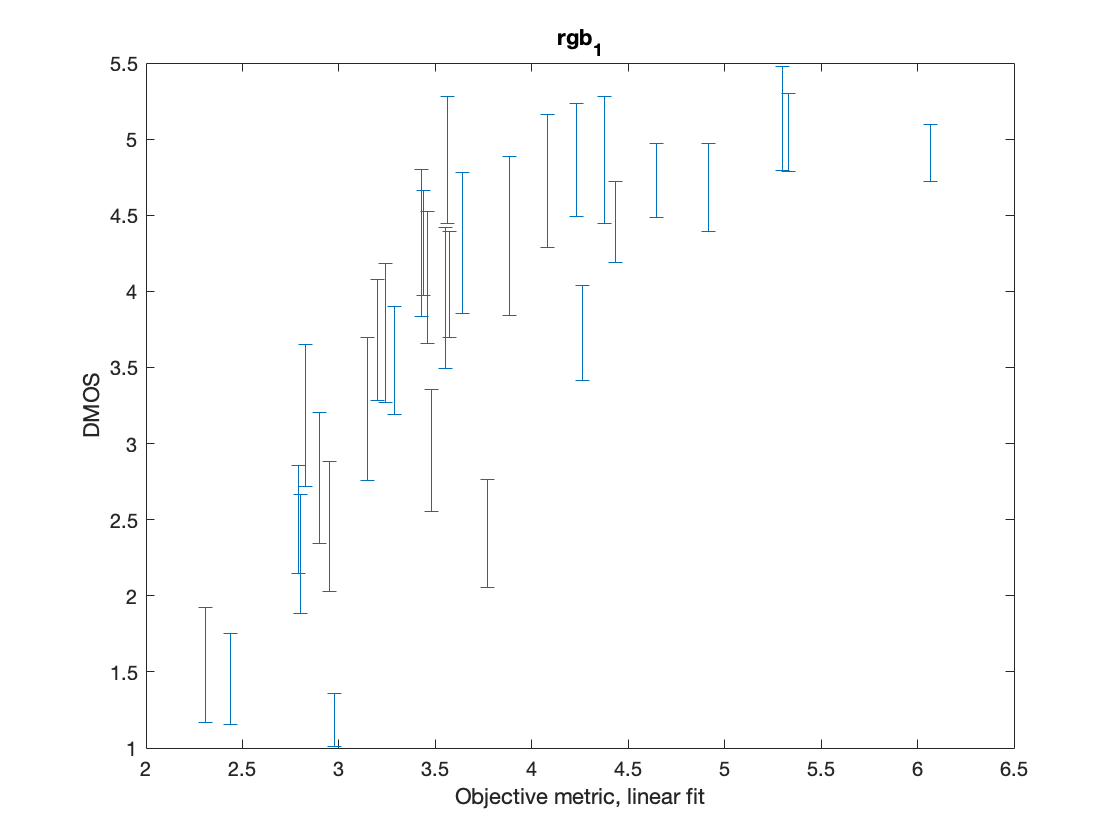
\includegraphics[width=\textwidth]{Figures/task3/rgb1_linear.png}
   \end{subfigure}
   
   \begin{subfigure}[b]{0.65\textwidth}
   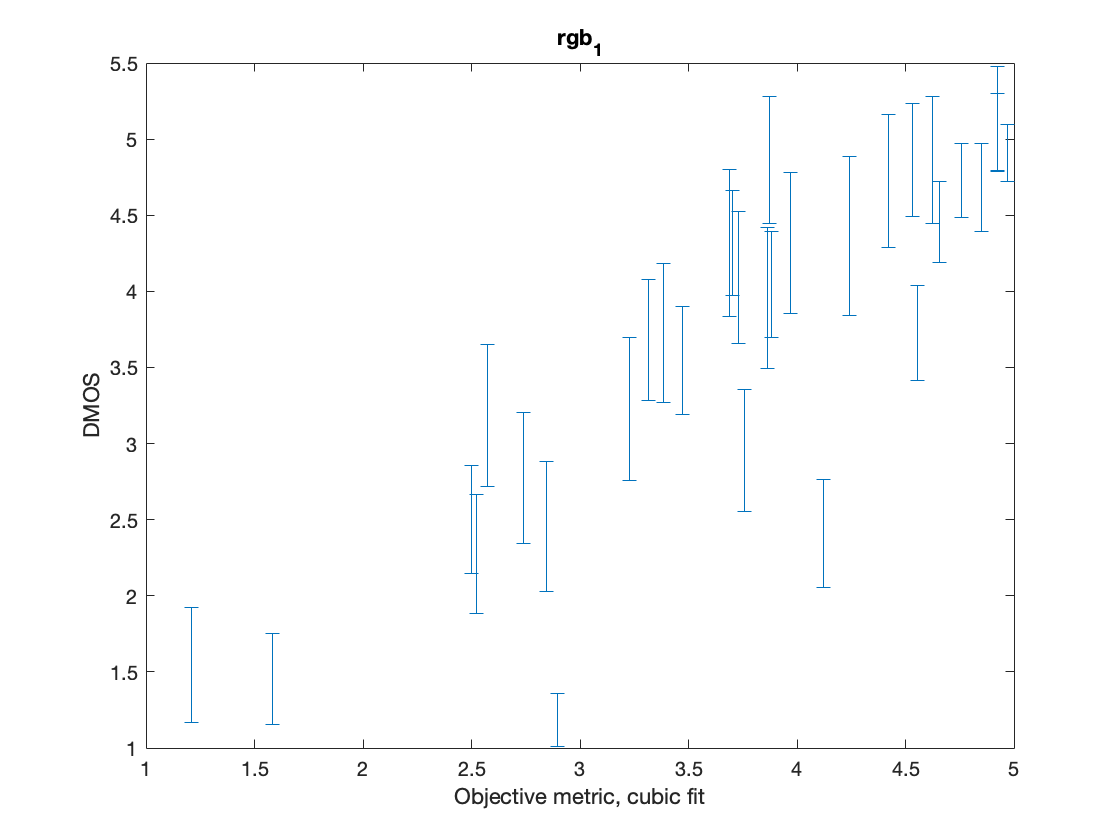
\includegraphics[width=\textwidth]{Figures/task3/rgb1_cubic.png}
   \end{subfigure}
    \label{fig:rgb1_fitted}
     \caption{DMOS vs. color PSNR in RGB using eq. 14 plain, linearly fitted, cubicly fitted.}
\end{figure}

\begin{figure}
    \centering
   \begin{subfigure}[b]{0.65\textwidth}
   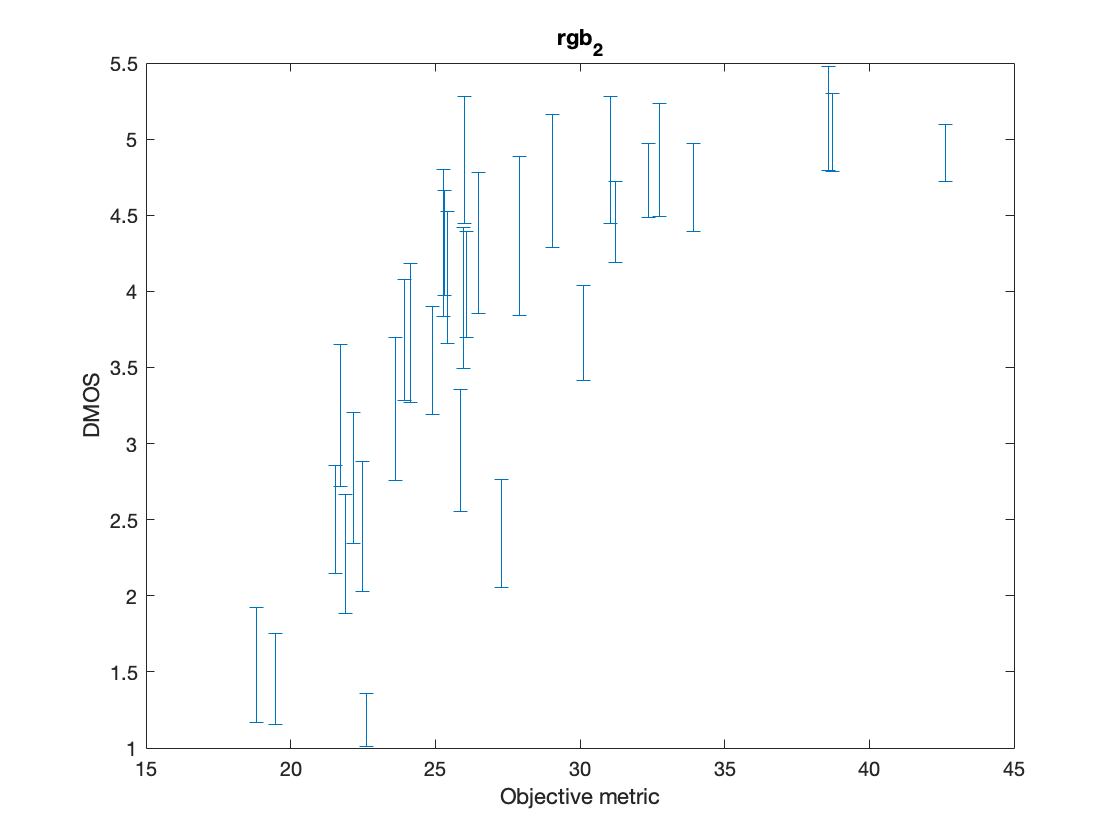
\includegraphics[width=\textwidth]{Figures/task3/rgb2.png}
   \end{subfigure}
   \begin{subfigure}[b]{0.65\textwidth}
   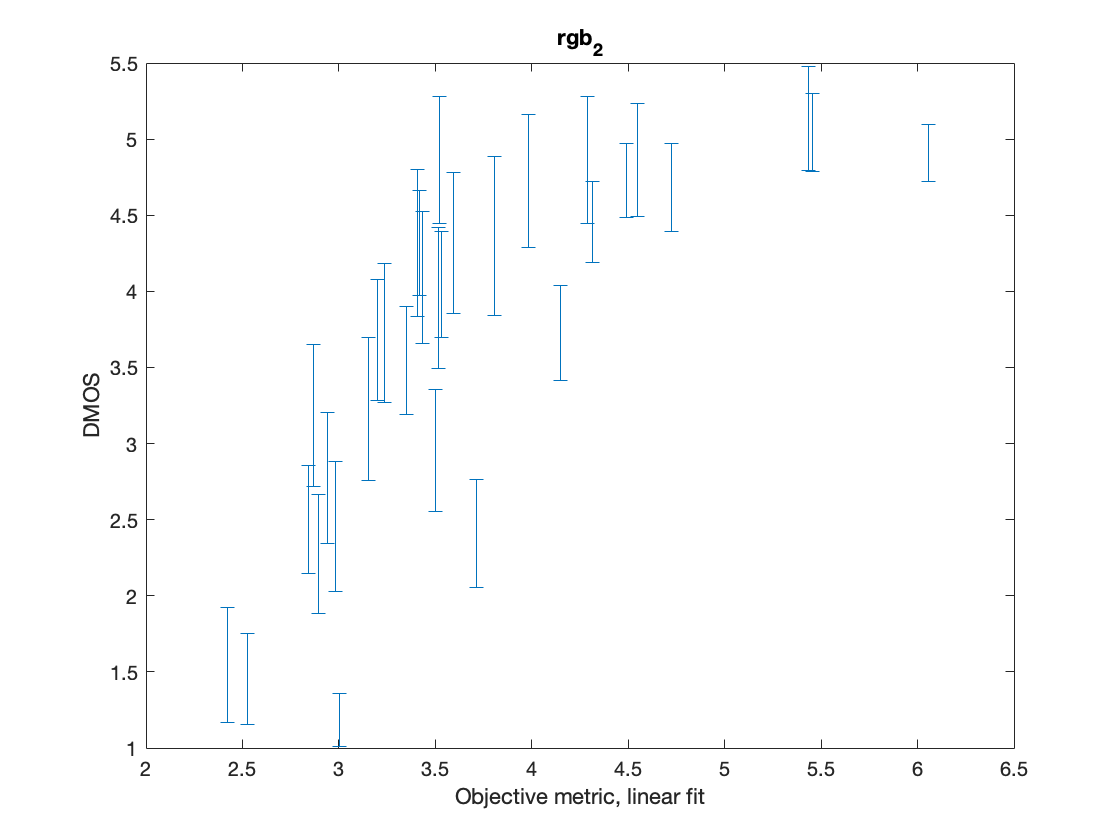
\includegraphics[width=\textwidth]{Figures/task3/rgb2_linear.png}
   \end{subfigure}
   \begin{subfigure}[b]{0.65\textwidth}
   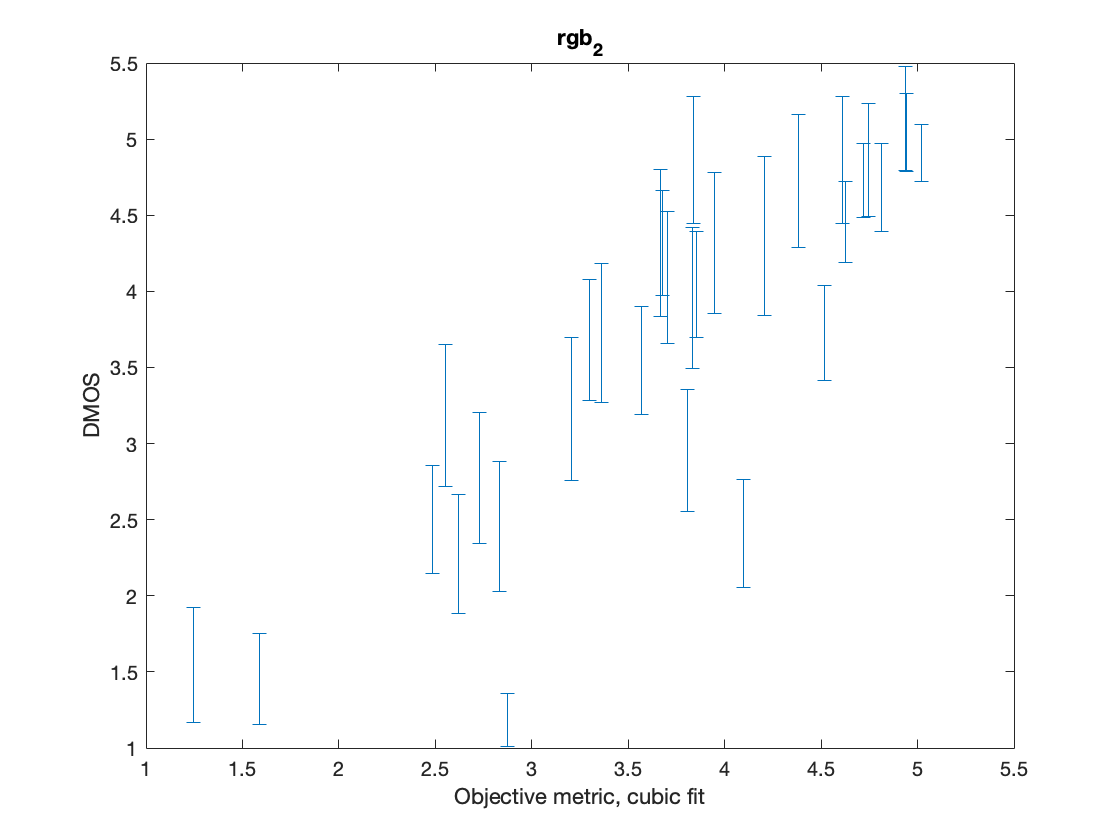
\includegraphics[width=\textwidth]{Figures/task3/rgb2_cubic.png}
   \end{subfigure}
    \caption{DMOS vs. color PSNR in RGB using eq. 15 plain, linearly fitted, cubicly fitted.}
    \label{fig:rgb2_fitted}
\end{figure}

\begin{figure}
    \centering
   \begin{subfigure}[b]{0.65\textwidth}
   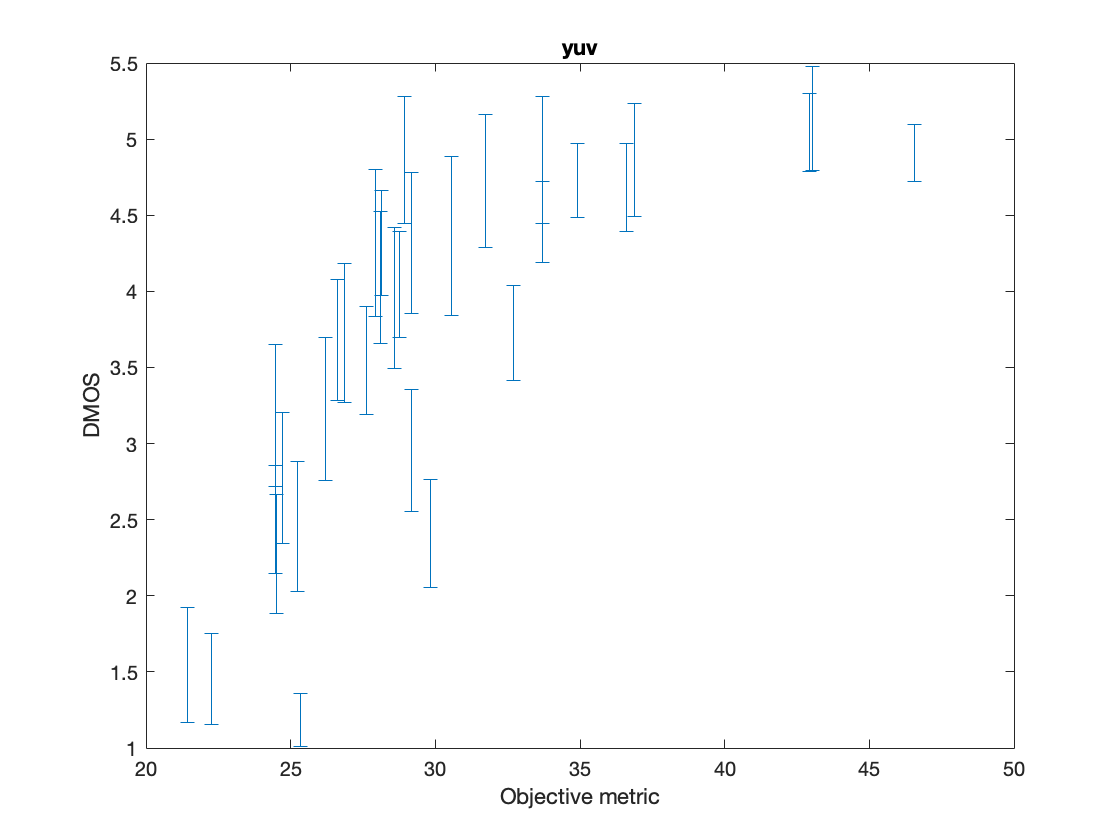
\includegraphics[width=\textwidth]{Figures/task3/yuv.png}
   \end{subfigure}
   \begin{subfigure}[b]{0.65\textwidth}
   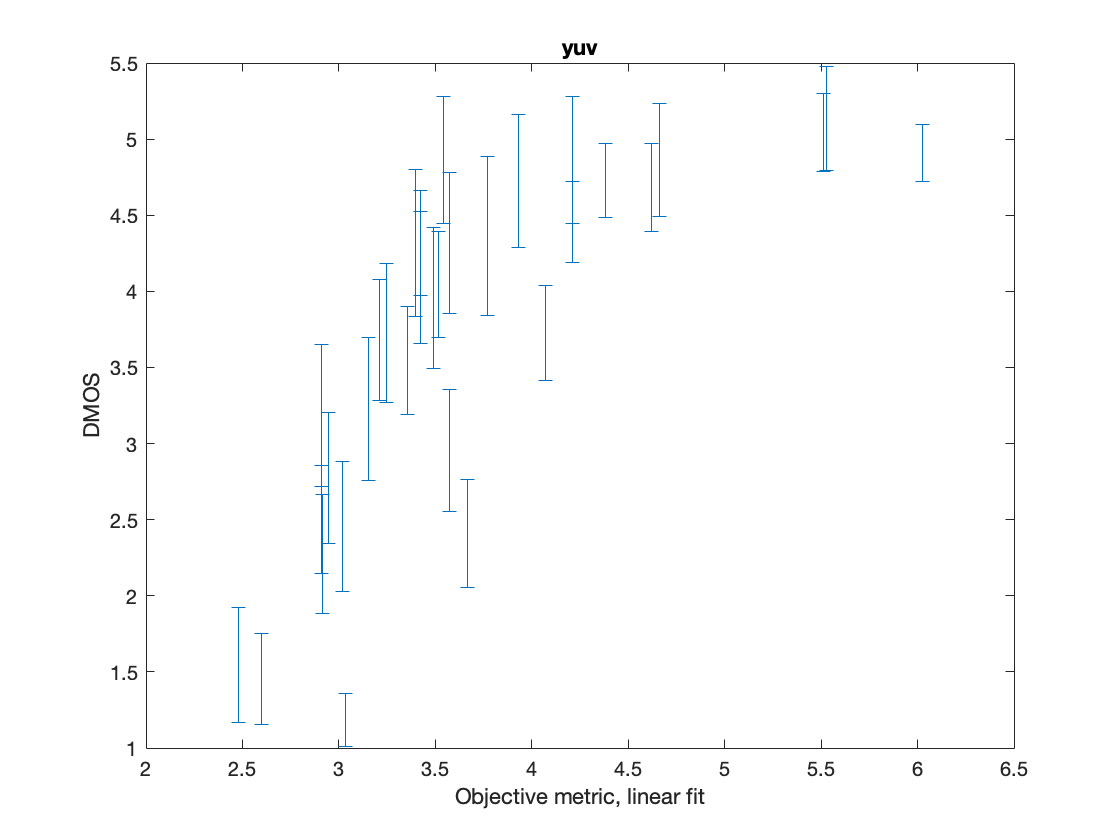
\includegraphics[width=\textwidth]{Figures/task3/yuv_linear.png}
   \end{subfigure}
   \begin{subfigure}[b]{0.65\textwidth}
   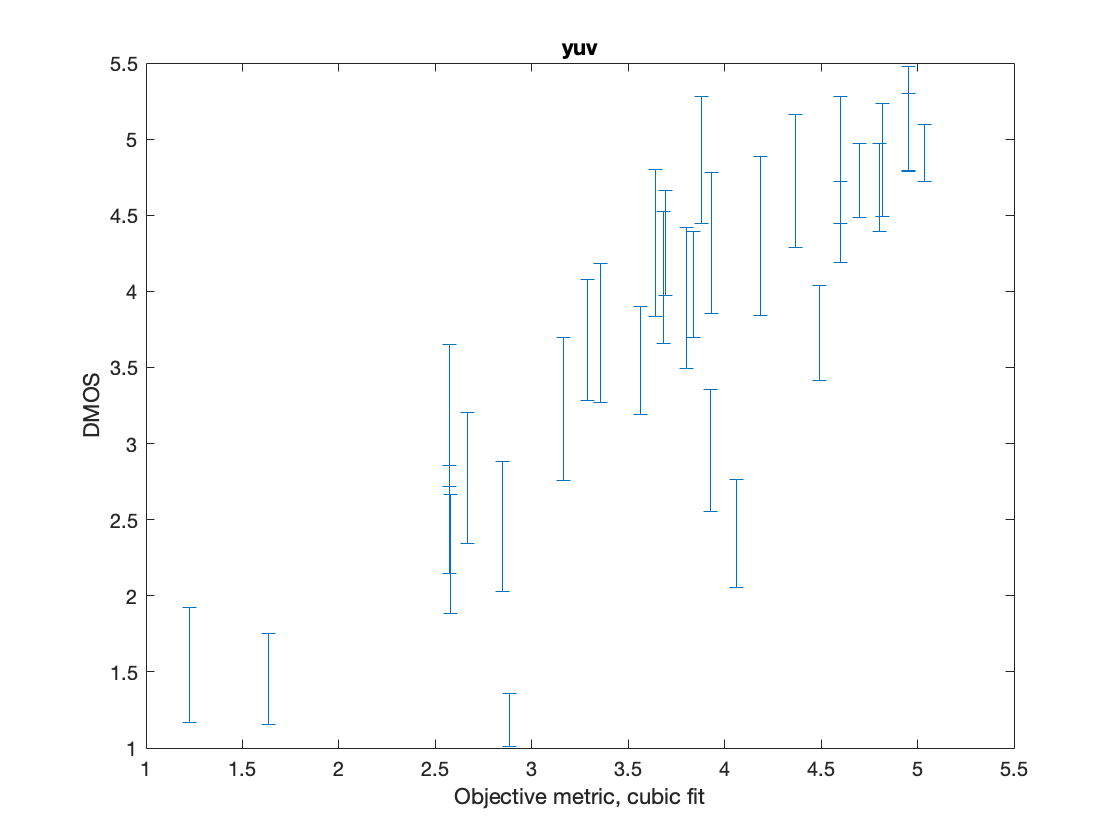
\includegraphics[width=\textwidth]{Figures/task3/yuv_cubic.png}
   \end{subfigure}%
    \caption{DMOS vs. color PSNR in YUV plain, linearly fitted, cubicly fitted.}
    \label{fig:yuv_fitted}
\end{figure}

\end{document}